\documentclass[hyperref=unicode,presentation,10pt]{beamer}

\usepackage[absolute,overlay]{textpos}
\usepackage{array}
\usepackage{graphicx}
\usepackage{adjustbox}
\usepackage[version=4]{mhchem}
\usepackage{chemfig}
\usepackage{caption}

%dělení slov
\usepackage{ragged2e}
\let\raggedright=\RaggedRight
%konec dělení slov

\addtobeamertemplate{frametitle}{
	\let\insertframetitle\insertsectionhead}{}
\addtobeamertemplate{frametitle}{
	\let\insertframesubtitle\insertsubsectionhead}{}

\makeatletter
\CheckCommand*\beamer@checkframetitle{\@ifnextchar\bgroup\beamer@inlineframetitle{}}
\renewcommand*\beamer@checkframetitle{\global\let\beamer@frametitle\relax\@ifnextchar\bgroup\beamer@inlineframetitle{}}
\makeatother
\setbeamercolor{section in toc}{fg=red}
\setbeamertemplate{section in toc shaded}[default][100]

\usepackage{fontspec}
\usepackage{unicode-math}

\usepackage{polyglossia}
\setdefaultlanguage{czech}

\def\uv#1{„#1“}

\mode<presentation>{\usetheme{default}}
\usecolortheme{crane}

\setbeamertemplate{footline}[frame number]

\title[Crisis]
{C2062 -- Anorganická chemie II}

\subtitle{(Uhlík, křemík,) germanium, cín, olovo a flerovium}
\author{Zdeněk Moravec, hugo@chemi.muni.cz \\ \adjincludegraphics[height=60mm]{img/IUPAC_PSP.jpg}}
\date{}

\begin{document}

\begin{frame}
	\titlepage
\end{frame}

\section{Uhlík}
\frame{
	\frametitle{}
	\begin{columns}
		\begin{column}{0.5\textwidth}
			\vfill
			\begin{itemize}
				\item \textbf{Uhlík}
				\item Prvek, se kterým se potkáváme v organické i anorganické chemii.
				\item Ve vesmíru se jedná o čtvrtý nejběžnější prvek, v lidském těle ho najdeme 18,5 \%.\footnote[frame]{\href{https://www.news-medical.net/life-sciences/What-Chemical-Elements-are-Found-in-the-Human-Body.aspx}{What Chemical Elements are Found in the Human Body?}}
				\item Základ organických sloučenin.
				\item V elementární formě se vyskytuje jako grafit a diamant.
				\item Mimo tyto běžné formy známe další allotropní modifikace, některé z nich mají velký potenciál do budoucna, některé se využívají už v dnešní době.
			\end{itemize}
			\vfill
		\end{column}
		\begin{column}{0.5\textwidth}
			\begin{figure}
				\adjincludegraphics[width=\textwidth]{img/Carbon_cycle.jpg}
				\caption*{Uhlíkový cyklus.\footnote[frame]{Zdroj: \href{https://commons.wikimedia.org/wiki/File:Carbon_cycle.jpg}{U.S. DOE/Commons}}}
			\end{figure}
		\end{column}
	\end{columns}
}

\subsection{Allotropické modifikace uhlíku}
\frame{
	\frametitle{}
	\vfill
	\begin{figure}
		\adjincludegraphics[height=0.7\textheight]{img/Eight_Allotropes_of_Carbon.png}
		\caption*{Allotropické modifikace uhlíku.\footnote[frame]{Zdroj: \href{https://commons.wikimedia.org/wiki/File:Eight_Allotropes_of_Carbon.png}{mstroeck/Commons}}}
	\end{figure}
	\vfill
}

\subsection{Diamant}
\frame{
	\frametitle{}
	\begin{columns}
		\begin{column}{0.65\textwidth}
			\vfill
			\textbf{Diamant}
			\begin{itemize}
				\item Jeden z nejtvrdších přírodních minerálů.
				\item Struktura se skládá z tetraedricky koordinovaných atomů sp$^3$ uhlíku.
				\item Vzniká v hloubkách 150--200~km za tlaku 4,5--6~GPa a teplot 900--1300~$^\circ$C.
				\item Chemicky je poměrně inertní.
				\item Diamanty se využívají ve šperkařství i v průmyslu.
				\item Některé diamanty mají polovodivé vlastnosti.
				\item Pro průmyslové aplikace se využívají přírodní diamanty nevhodné pro šperky nebo umělé diamanty.
			\end{itemize}
			\vfill
		\end{column}
		\begin{column}{0.4\textwidth}
			\begin{figure}
				\adjincludegraphics[width=0.65\textwidth]{img/Diamonds_from_Catoka_mine_4.jpg}\caption*{Diamanty z Angoly.\footnote[frame]{Zdroj: \href{https://commons.wikimedia.org/wiki/File:Diamonds_from_Catoka_mine_4.jpg}{Helgi/Commons}}}
				\adjincludegraphics[width=0.6\textwidth]{img/Carbon_lattice_diamond.png}
				\caption*{Krystalová struktura diamantu.\footnote[frame]{Zdroj: \href{https://commons.wikimedia.org/wiki/File:Carbon_lattice_diamond.png}{YassineMrabet/Commons}}}
			\end{figure}
		\end{column}
	\end{columns}
}

\subsection{Syntetické diamanty}
\frame{
	\frametitle{}
	\begin{columns}
		\begin{column}{0.65\textwidth}
			\vfill
			\begin{itemize}
				\item HPHT -- High Pressure, High Temperature -- uhlík je v přítomnosti kovového katalyzátoru zahříván na vysoké teploty. Proces probíhá za vysokého tlaku.
				\item CVD -- jako zdroj uhlíku se využívají plynné uhlovodíky. Tato metoda se využívá hlavně pro laboratorní přípravu diamantů.
				\item Ultrazvuková kavitace (sonochemie) -- proces probíhá za laboratorní teploty a tlaku. Do suspenze grafitu v organickém rozpouštědle je zaváděn ultrazvuk. Vznikají diamanty o velikosti mikrometrů.
			\end{itemize}
			\vfill
		\end{column}
		\begin{column}{0.4\textwidth}
			\begin{figure}
				\adjincludegraphics[width=0.7\textwidth]{img/HPHTdiamonds2.jpg}
				\caption*{HPHT diamanty.\footnote[frame]{Zdroj: \href{https://commons.wikimedia.org/wiki/File:HPHTdiamonds2.JPG}{Materialscientist/Commons}}}
				\adjincludegraphics[width=.85\textwidth]{img/BARS4.png}
				\caption*{BARS systém pro přípravu diamantů.\footnote[frame]{Zdroj: \href{https://commons.wikimedia.org/wiki/File:BARS4.svg}{Heribero Arribas Abato/Commons}}}
			\end{figure}
		\end{column}
	\end{columns}
}

\subsection{Nanodiamanty}
\frame{
	\frametitle{}
	\vfill
	\begin{itemize}
		\item Velmi malé syntetické diamanty, jejich velikost se pohybuje mezi 4 a 100~nm.\footnote[frame]{\href{https://www.osel.cz/11343-k-cemu-vsemu-se-muzou-hodit-nanodiamanty.html}{K čemu všemu se můžou hodit nanodiamanty?}}
		\item Díky malým rozměrům mají poměrně unikátní vlastnosti, které lze ovlivňovat.\footnote[frame]{\href{https://www.sigmaaldrich.com/technical-documents/articles/technology-spotlights/monodispersed-nanodiamonds-applications.html}{Monodispersed Nanodiamonds and their Applications}}
		\item \textit{Detonační nanodiamanty} -- vznikají explozí vhodné výbušniny (TNT, hexogen) v uzavřeném reaktoru.
		\item Jejich dopováním borem lze získat slibné polovodivé materiály, které by mohly umožnit další miniaturizaci elektroniky.
		\item Dopováním dusíkem získáme nanodiamanty s fluorescenčními vlastnostmi.
		\item Díky jejich biokompatibilitě je možné je využít i pro medicinální účely, např. k transportu léčiva, jako fluorescenční sondy.
	\end{itemize}
	\vfill
}

\subsection{Grafit}
\frame{
	\frametitle{}
	\vfill
	\begin{figure}
		\adjincludegraphics[height=0.65\textheight]{img/Diamond_and_graphite2.jpg}
		\caption*{Srovnání diamantu a grafitu.\footnote[frame]{Zdroj: \href{https://commons.wikimedia.org/wiki/File:Diamond_and_graphite2.jpg}{Itub/Commons}}}
	\end{figure}
	\vfill
}

\frame{
	\frametitle{}
	\begin{columns}
		\begin{column}{0.5\textwidth}
			\vfill
			\textbf{Grafit}
			\begin{itemize}
				\item Měkký, na omak mastný, dobře štěpný, vede dobře teplo i elektrický proud.
				\item Struktura se skládá z vrstev atomů sp$^2$ uhlíku. Atomy ve vrstvách jsou vázány kovalentně, vrstvy jsou drženy van der Waalsovými vazbami.
				\item Využívá se jako mazivo, k psaní, jako materiál elektrod i do vyzdívek pecí.
				\item Reaguje s \ce{HNO3} za vyšší teploty. Lze připravit interkaláty grafitu.
			\end{itemize}
			\vfill
		\end{column}
		\begin{column}{0.5\textwidth}
			\begin{figure}
				\adjincludegraphics[width=0.8\textwidth]{img/Graphit_gitter.png}
				\caption*{Struktura grafitu.\footnote[frame]{Zdroj: \href{https://commons.wikimedia.org/wiki/File:Graphit_gitter.png}{Anton/Commons}}}
			\end{figure}
		\end{column}
	\end{columns}
}

\subsection{Interkaláty grafitu}
\frame{
	\frametitle{}
	\begin{columns}
		\begin{column}{0.5\textwidth}
			\vfill
			\begin{itemize}
				\item Sloučeniny s obecným vzorcem \ce{CX_m}, vznikají zavedením iontů \ce{X^{n+}} nebo \ce{X^{n-}} mezi vrstvy grafitu.
				\item Interkaláty grafitu se liší zbarvením i elektrickými vlastnostmi. Připravují se reakcí grafitu se silnými oxidačními nebo redukčními činidly, např. K, \ce{O2 + H2SO4}.
				\item Mezi nejlépe prozkoumané systémy patří interkaláty s draslíkem, např. \ce{KC8, KC24, KC36, KC48} a \ce{KC60}.
			\end{itemize}
			\vfill
		\end{column}
		\begin{column}{0.5\textwidth}
			\begin{figure}
				\adjincludegraphics[width=0.9\textwidth]{img/Potassium-graphite-xtal-3D-SF-A.png}
				\caption*{Krystalová struktura \ce{KC8}, fialové kuličky představují ionty \ce{K+}.\footnote[frame]{Zdroj: \href{https://commons.wikimedia.org/wiki/File:Potassium-graphite-xtal-3D-SF-A.png}{Ben Mills/Commons}}}
			\end{figure}
		\end{column}
	\end{columns}
}

\frame{
	\frametitle{}
	\begin{columns}
		\begin{column}{0.6\textwidth}
			\vfill
			\begin{itemize}
				\item \ce{CaC6} je supravodivý s hodnotou kritické teploty T$_C$~=~11,5~K (15,1~K při 8~GPa).\footnote[frame]{\href{https://dx.doi.org/10.1088/1468-6996/9/4/044102}{Synthesis and superconducting properties of \ce{CaC6}}}
				\item Nejprve se v suchém boxu s čistým argonem smísí vápník s lithiem v poměru 3-4:1. Tato směs taje v rozmezí teplot 400-450~$^\circ$C, což je dostatečně nízká teplota, aby se předešlo vzniku karbidu vápníku.
				\item Směs je uzavřena do trubkové pece a~roztavena.
				\item K tavenině se přidá grafit a zahřívání probíhá v atmosféře argonu při teplotě 350~$^\circ$C po dobu 10 dní.
			\end{itemize}
			\vfill
		\end{column}
		\begin{column}{0.4\textwidth}
			\begin{figure}
				\adjincludegraphics[width=\textwidth]{img/Glovebox.jpg}
				\caption*{Suchý box.\footnote[frame]{Zdroj: \href{https://commons.wikimedia.org/wiki/File:Glovebox.jpg}{Rune.welsh/Commons}}}
			\end{figure}
		\end{column}
	\end{columns}
}

\frame{
	\frametitle{}
	\begin{figure}
		\adjincludegraphics[height=.7\textheight]{img/Tube-furnace.jpg}
		\caption*{Příprava \ce{KC8} probíhá v trubkové peci.\footnote[frame]{Zdroj: \href{https://commons.wikimedia.org/wiki/File:Horno_tubular.jpg}{Manuel Almagro Rivas/Commons}}}
	\end{figure}
}

\subsection{Oxid grafitu}
\frame{
	\frametitle{}
	\vfill
	\textbf{Oxid grafitu}
	\begin{itemize}
		\item Někdy se označuje jako kyselina grafitová. Skládá se z uhlíku, kyslíku a vodíku, jejich poměr je proměnný.
		\item Poprvé byl připraven roku 1859 reakcí grafitu s chlorečnanem draselným a~dýmavou kyselinou dusičnou.\footnote[frame]{\href{https://doi.org/10.1098/rstl.1859.0013}{On the atomic weight of graphite}}
		\item V roce 1957 byla vyvinuta bezpečnější a účinější metoda oxidace označovaná jako \textit{Hummerova metoda}. Jako oxidační činidlo je využívána směs koncentrované kyseliny sírové, dusičnanu sodného a manganistanu draselného.\footnote[frame]{\href{https://doi.org/10.1021/ja01539a017}{Preparation of Graphitic Oxide}}
		\item Struktura oxidu grafitu je závislá na metodě přípravy a stupni oxidace. Zachovává si vrstevnatý charakter grafitu, ale vzdálenost mezi rovinami je zhruba dvakrát vyšší než u grafitu.
		\item Je hydrofilní a snadno se hydratuje stykem s vodou nebo vodní parou.
	\end{itemize}
	\vfill
}

\subsection{Grafen}
\frame{
	\frametitle{}
	\vfill
	\begin{itemize}
		\item \textbf{Grafen} -- monovrstva tvořená sp$^2$ uhlíky.
		\item Poprvé byl připraven v roce 2004 exfoliací grafitu pomocí lepící pásky.\footnote[frame]{\href{https://www.idnes.cz/zpravy/zahranicni/nobelovu-cenu-za-fyziku-dostali-vedci-za-vyzkum-supertenkeho-uhliku.A101005_120031_zahranicni_aha}{Nobelovu cenu za fyziku dostali vědci za výzkum supertenkého uhlíku}} V roce 2010 byla za tento objev udělena Nobelova cena za fyziku.\footnote[frame]{\href{https://www.nobelprize.org/prizes/physics/2010/press-release/}{The Nobel Prize in Physics 2010}}
		\item V roce 2008 byl grafen nejdražším materiálem světa, 1~cm$^2$ stál zhruba \$100~000~000.
		\item V roce 2009 klesla cena na \$100/cm$^2$. Příčinou poklesu ceny byla optimalizace exfoliačních metod pro velkoobjemovou syntézu a k vývoji CVD metody výroby grafenu.
		\item Grafen je 200$\times$ pevnější než ocel, zároveň je ale i tvrdší a lehčí.
		\item Pohyblivost elektronů v grafenu je řádově vyšší než v křemíku, proto by mohl být výhodný pro konstrukci čipů.
		\item V závislosti na struktuře může vystupovat jako izolant, polovodič, vodič i supravodič.
	\end{itemize}
	\vfill
}

\frame{
	\frametitle{}
	\begin{columns}
		\begin{column}{0.5\textwidth}
			\begin{figure}
				\adjincludegraphics[height=0.45\textheight]{img/Graphen.jpg}
				\caption*{Grafenová vrstva.\footnote[frame]{Zdroj: \href{https://commons.wikimedia.org/wiki/File:Graphen.jpg}{AlexanderAlUS/Commons}}}
			\end{figure}
		\end{column}
		\begin{column}{0.5\textwidth}
			\begin{figure}
				\adjincludegraphics[height=0.45\textheight]{img/Graphene.jpg}
				\caption*{Grafen připravený CVD na měděném substrátu.\footnote[frame]{Zdroj: \href{https://commons.wikimedia.org/wiki/File:Graphene.jpg}{Tavo Romann/Commons}}}
			\end{figure}
		\end{column}
	\end{columns}
}

\subsection{Fullereny}
\frame{
	\frametitle{}
	\begin{columns}
		\begin{column}{0.65\textwidth}
			\vfill
			\begin{itemize}
				\item \textbf{Fullereny}
				\item Uzavřené, prostorové molekuly skládající se z atomů uhlíku.
				\item V jejich dutině (kavitě) je možno uzavřít atomy nebo molekuly.
				\item Jejich existence byla předpovězena v roce 1970, první syntéza byla publikována až v roce 1980.
				\item Roku 1985 byly připraveny a identifikovány fullereny \ce{C60} a \ce{C70}, roku 1996 byla udělena Nobelova cena za výzkum v této oblasti.
				\item Nejznámější a nejstabilnější je tzv. \textit{Buckminsterfulleren} \ce{C60}.
			\end{itemize}
			\vfill
		\end{column}
		\begin{column}{0.4\textwidth}
			\begin{figure}
				\adjincludegraphics[width=.8\textwidth]{img/Buckminsterfullerene-2D-skeletal.png}
				\adjincludegraphics[width=.8\textwidth]{img/C60_Fullerene_solution.jpg}
				\caption*{Roztok fullerenu \ce{C60} v benzenu.\footnote[frame]{Zdroj: \href{https://commons.wikimedia.org/wiki/File:C60_Fullerene_solution.jpg}{Alpha Six/Commons}}}
			\end{figure}
		\end{column}
	\end{columns}
}

\frame{
	\frametitle{}
	\begin{columns}
		\begin{column}{0.65\textwidth}
			\vfill
			\begin{itemize}
				\item Standardně se fullereny připravují působením elektrického oblouku na grafit v~atmosféře helia.
				\item Lze je získat i ozařováním polycyklických aromatických uhlovodíků laserem.
				\item Všechny metody syntézy poskytují směs fullerenů, kterou je nutné následně separovat pomocí chromatografických metod.
			\end{itemize}
			\begin{figure}
				\adjincludegraphics[width=.7\textwidth]{img/PAHs.png}
			\end{figure}
			\vfill
		\end{column}
		\begin{column}{0.4\textwidth}
			\begin{figure}
				\adjincludegraphics[width=\textwidth]{img/Lichtbogen_3000_Volt.jpg}
				\caption*{Obloukový výboj.\footnote[frame]{Zdroj: \href{https://commons.wikimedia.org/wiki/File:Lichtbogen_3000_Volt.jpg}{Achgro/Commons}}}
			\end{figure}
		\end{column}
	\end{columns}
}

\frame{
	\frametitle{}
	\vfill
	\begin{itemize}
		\item Skládají se z pěti a šestičlenných kruhů tvořených $sp^2$ uhlíkem.
		\item Jejich základní vlastnosti jsou:
		\begin{itemize}
			\item Vysoká elektronová afinita.
			\item Strukturní stabilita.
			\item Vysoký měrný povrch.
		\end{itemize}
		\item Těchto vlastností se využívá např. při konstrukci chemických a biologických senzorů.
		\item Známe dva druhy derivátů fullerenů:
		\begin{itemize}
			\item \textit{Exohedrální} -- připojení funkční skupiny na povrch fullerenové klece.
			\item \textit{Endohedrální} -- vložení atomu nebo malé molekuly (\ce{H2}, \ce{H2O}) dovnitř fullerenové klece, např. $\text{H}_2@\text{C}_{60}$.
		\end{itemize}
	\end{itemize}
	\vfill
}

\frame{
	\frametitle{}
	\vfill
	\begin{columns}
		\begin{column}{.5\textwidth}
			\begin{figure}
				\adjincludegraphics[height=.3\textheight]{img/fullerenes/Endohedral_fullerene.png}
				\caption*{Endohedrální derivát fullerenu.\footnote[frame]{Zdroj: \href{https://commons.wikimedia.org/wiki/File:Endohedral_fullerene.png}{Hajv01/Commons}}}
			\end{figure}
		\end{column}
		\begin{column}{.5\textwidth}
			\begin{figure}
				\adjincludegraphics[height=.3\textheight]{img/fullerenes/Ir-fullerene.png}
				\caption*{Exohedrální derivát fullerenu.\footnote[frame]{Zdroj: \href{https://commons.wikimedia.org/wiki/File:Ir-fullerene.svg}{Xhmikos/Commons}}}
			\end{figure}
		\end{column}
	\end{columns}
	\begin{figure}
		\adjincludegraphics[width=.5\textwidth]{img/fullerenes/Fullerene_dumbbell.jpg}
		\caption*{Exohedrální derivát fullerenu.\footnote[frame]{Zdroj: \href{https://commons.wikimedia.org/wiki/File:Fullerene_dumbbell.jpg}{123 nano/Commons}}}
	\end{figure}
	\vfill
}

\frame{
	\frametitle{}
	\vfill
	\begin{figure}
		\adjincludegraphics[height=.4\textheight]{img/fullerenes/Molecular surgery.png}
		\adjincludegraphics[height=.32\textheight]{img/fullerenes/Molecular surgery2.png}
		\caption*{Molekulární chirurgie.\footnote[frame]{Zdroj: \href{https://doi.org/10.1039/B811738A}{Surgery of fullerenes}}}
	\end{figure}
	\vfill
}

\frame{
	\frametitle{}
	\begin{columns}
		\begin{column}{0.5\textwidth}
			\vfill
			\begin{itemize}
				\item Využití v lékařství:
				\begin{itemize}
					\item Antioxidanty
					\item Doprava léčiv na místo působení
					\item Diagnostika
					\item Antivirové látky
				\end{itemize}
				\item V kosmetice se využívají např. jako látky zpomalující stárnutí, díky jejich antioxidačním vlastnostem.
				\item Suchá maziva pro ložiska, převodovky, pumpy, atd.
			\end{itemize}
			\vfill
		\end{column}
		\begin{column}{0.5\textwidth}
			\begin{figure}
				\adjincludegraphics[width=.9\textwidth]{img/fullerenes/Buckminsterfullerene_Model_in_Red_Beads.jpg}
				\caption*{Model fullerenu v Muzeu Nobelových cen.\footnote[frame]{Zdroj: \href{https://commons.wikimedia.org/wiki/File:Buckminsterfullerene_Model_in_Red_Beads.jpg}{Wing-Chi Poon/Commons}}}
			\end{figure}
		\end{column}
	\end{columns}
}

\subsection{Uhlíkové nanotrubice}
\frame{
	\frametitle{}
			\vfill
			\begin{itemize}
				\item Válcovité molekuly tvořené uhlíkem. Jejich průměr se pohybuje v nm.
				\item Podle počtu stěn rozlišujeme:
				\begin{itemize}
					\item Jednostěnné uhlíkové nanotrubice (SWCNT - Single-Walled Carbon NanoTubes)
					\item Dvoustěnné uhlíkové nanotrubice (DWCNT - Double-Walled Carbon NanoTubes)
					\item Vícestěnné uhlíkové nanotrubice (MWCNT - Multi-Walled Carbon NanoTubes)
				\end{itemize}
				\item První uhlíková vlákna o průměru 50~nm byla připravena v roce 1952.
				\item SWCNT byly připraveny až v roce 1993.
				\item V obloukovém výboji vznikají hlavně MWCNT, větší množství SWCNT lze připravit laserovým odpařováním (ablací) uhlíku.\footnote[frame]{\href{https://www.intechopen.com/chapters/72939}{Carbon Nanotubes: Synthesis, Properties and Applications}}
			\end{itemize}
			\vfill
}

\frame{
	\frametitle{}
	\begin{columns}
		\begin{column}{0.5\textwidth}
			\begin{figure}
				\adjincludegraphics[width=\textwidth]{img/Multi-walled_Carbon_Nanotube.png}
				\caption*{Model vícestěnné uhlíkové nanotrubice.\footnote[frame]{Zdroj: \href{https://commons.wikimedia.org/wiki/File:Multi-walled_Carbon_Nanotube.png}{Eric Wieser/Commons}}}
			\end{figure}

		\end{column}

		\begin{column}{0.5\textwidth}
			\begin{figure}
				\adjincludegraphics[width=.9\textwidth]{img/Multi-walled_carbon_nanotube.jpg}
				\caption*{TEM snímek vícestěnné uhlíkové nanotrubice.\footnote[frame]{Zdroj: \href{https://commons.wikimedia.org/wiki/File:Multi-walled_carbon_nanotube.jpg}{Anna-Versh/Commons}}}
			\end{figure}
		\end{column}
	\end{columns}
}

\frame{
	\frametitle{}
	\vfill
	\begin{itemize}
		\item Youngův modul CNT je okolo 270--950~GPa (pro ocel se pohybuje okolo 200~GPa).
		\item V roce 1979 byla vydána kniha \textit{Rajské fontány} A. C. Clarka, kde popisuje kosmický výtah, jehož tažné lano je tvořeno uhlíkem, resp. jednorozměrným diamantem.\footnote[frame]{\href{https://www.cbdb.cz/kniha-3198-rajske-fontany-the-fountains-of-paradise}{Rajské fontány}}
		\item Chemicky jsou stabilní, mají vysoký měrný povrch, což umožňuje jejich dopování jinými prvky.
		\item Jsou dobrými vodiči tepla a mají vysokou teplotní stabilitu, degradace nastává při teplotách vyšších než 500~$^\circ$C.
		\item Z hlediska elektrické vodivosti se mohou chovat jako polovodiče, kovy i supravodiče, v závislosti na jejich struktuře.
		\item Lze je připravit působením elektrického oblouku, laserovou ablací nebo pomocí CVD.
		\item Byly objeveny i v historické damascénské oceli.\footnote[frame]{\href{https://www.thevintagenews.com/2017/04/03/damascus-blacksmiths-had-made-steel-blades-with-carbon-nanotubes-long-before-they-were-scientifically-discovered/}{Damascus blacksmiths had made steel blades with carbon nanotubes long before they were scientifically discovered}}
	\end{itemize}
	\vfill
}

%Křemík, polovodiče, zonální tavba, silany
\section{Křemík}
\frame{
	\frametitle{}
	\vfill
	\begin{columns}
		\begin{column}{0.65\textwidth}
			\begin{itemize}
				\item \textbf{Křemík} je velmi zajímavý prvek jak z hlediska chemických vlastností, tak i z hlediska praktických aplikací.
				\item Chemicky je sice podobný ostatním prvkům 14. skupiny, ale v~mnoha ohledech se od nich i odlišuje.\footnote[frame]{\textit{Je na místě plísnit chemika, který se pokouší aplikovat úspěch organické chemie na studium polysilanů, neboť se chová jako ten, jenž dojí koně, a přitom rajtuje krávu.} \href{https://academictree.org/chemistry/publications.php?pid=76303}{Grant Urry}}
				\item Minerály křemíku doprovázejí lidstvo od samého počátku.
				\item Čistý křemík připravil až v roce 1823 J. J. Berzelius redukcí \ce{K2[SiF6]} taveninou draslíku:
				\item \ce{K2[SiF6] + 4 K ->[70 $^\circ$C] Si + 6 KF}
			\end{itemize}
		\end{column}

		\begin{column}{0.4\textwidth}
			\begin{figure}
				\adjincludegraphics[width=.75\textwidth]{img/Berzelius.jpg}
				\caption*{Jöns Jakob Berzelius.\footnote[frame]{Zdroj: \href{https://commons.wikimedia.org/wiki/File:Berzelius.jpg}{Commons}}}
			\end{figure}
		\end{column}
	\end{columns}
	\vfill
}

\frame{
	\frametitle{}
	\vfill
	\begin{columns}
		\begin{column}{0.75\textwidth}
			\begin{itemize}
				\item Surový křemík se vyrábí redukcí křemenného písku koksem:
				\item \ce{SiO2 + 2 C -> Si + 2 CO}
				\item \ce{2 SiC + SiO2 -> 3 Si + 2 CO}
				\item Čistý křemík se získává z těkavých sloučenin, které je možné přečistit destilací, \ce{SiCl4} nebo \ce{SiHCl3}.
				\item \ce{SiCl4 + 2 Zn -> Si + 2 ZnCl2}
				\item Získaný houbovitý křemík se přetaví do válcového krystalu, který se čistí \textit{zonální tavbou}.
				\item Alternativou je rozklad jodidu křemičitého na žhaveném wolframovém vlákně.
				\item \ce{SiI4 + 2 H2 ->[W] Si + 4 HI}
				\item Vysoce čistý křemík se využívá v polovodičovém průmyslu.
			\end{itemize}
		\end{column}

		\begin{column}{0.4\textwidth}
			\begin{figure}
				\adjincludegraphics[height=.35\textheight]{img/Silicon.jpg}
				\caption*{Vysoce čistý křemík.\footnote[frame]{Zdroj: \href{https://commons.wikimedia.org/wiki/File:Silicon.jpg}{Jurii/Commons}}}
			\end{figure}
		\end{column}
	\end{columns}
	\vfill
}

\frame{
	\frametitle{}
	\vfill
	\textbf{Zonální tavba}
	\begin{itemize}
		\item Tato metoda se využívá na čištění krystalických látek.\footnote{\href{https://csacg.fzu.cz/func/viewpdf.php?file=2000_34Drapala.pdf}{Zonální tavba jako krystalizační a rafinační metoda}}
		\item Je založeno na opakovaném roztavení části krystalického materiálu.
		\item Po roztavení dochází k pohybu příměsí směrem dolů.
		\item Ochlazením vzniká z taveniny polykrystalického materiálu monokrystal.
		\item Opakováním tohoto procesu zvyšujeme čistotu materiálu.
	\end{itemize}
	\begin{figure}
		\adjincludegraphics[width=.6\textwidth]{img/Zone-refining.jpg}
		\caption*{Zonální tavba.\footnote[frame]{Zdroj: \href{https://commons.wikimedia.org/wiki/File:Zone-refining.jpg}{Dbuckingham42/Commons}}}
	\end{figure}
	\vfill
}

\frame{
	\frametitle{}
	\vfill
	\textbf{Van Arkelova-de Boerova metoda}.
	\begin{itemize}
		\item Tato metoda se používá pro přípravu nejen křemíku, ale i velmi čistého zirkonia, titanu, hafnia a vanadu.
		\item Jedinou podmínkou pro použití této metody je existence těkavého halogenidu daného kovu.
		\item Surový materiál je zahříván ve vakuu s parami halogenu.
		\item Vzniklý těkavý halogenid je veden na žhavené vlákno, kde se rozkládá za vzniku čistého kovu.
		\item Nečistoty zůstávají v pevné fázi v zásobníku.
	\end{itemize}
	\vfill
}

\frame{
	\frametitle{}
	\vfill
	\begin{figure}
		\adjincludegraphics[height=.7\textheight]{img/Van-Arkel-de-Boer-Apparat.png}
		\caption*{1 - přívod vakua; 2 - molybdenová elektroda; 3 - molybdenová síť; 4 - zásobník surového materiálu; 5 - wolframové vlákno\footnote[frame]{Zdroj: \href{https://commons.wikimedia.org/wiki/File:Van-Arkel-de-Boer-Apparat.png}{	Roland Mattern/Commons}}}
	\end{figure}
	\vfill
}

\frame{
	\frametitle{}
	\vfill
	\begin{itemize}
		\item V roce 2019 bylo vyrobeno téměř 8,5 milónů tun křemíku.\footnote{\href{https://www.statista.com/statistics/573585/global-silicon-production/}{Production of silicon worldwide from 2010 to 2020}}
		\item Velká část je zpracovávána na ferrosilicia, což jsou slitiny železa a křemíku.
		\item Využívá se jako zdroj křemíku pro redukci oxidů kovů a pro přípravu deoxygenované oceli.
		\item Slouží i jako zdroj křemíku pro průmyslovou přípravu trichlorsilanu, \ce{SiHCl3}.
		\item \ce{Si + 3 HCl -> SiHCl3 + H2}
		\item Dříve se tato slitina využívala i jako bezpečný zdroj vodíku pro armádní účely:\footnote{\href{https://ntrs.nasa.gov/api/citations/19930091069/downloads/19930091069.pdf}{The ferrosilicon process for the generation of hydrogen}}
		\item \ce{2 NaOH + Si + H2O -> Na2SiO3 + 2 H2}
		\item Velká část křemíku se využívá v polovodičovém průmyslu.
	\end{itemize}
	\vfill
}

\subsection{Polovodiče}
\frame{
	\frametitle{}
	\vfill
	\begin{itemize}
		\item[1821] první polovodič, Thomas Seebeck
		\item[1907] objev elektroluminiscence
		\item[1927] objev LED
		\item[1940] objev PN přechodu
		\item[1947] první tranzistor
		\item[1953] objev elektroluminiscence u organických látek
		\item[1959] bipolární integrovaný obvod, Texas Instruments a Fairchild Semiconductor
		\item[1960] objev MOS tranzistoru
		\item[1962] LED emitující viditelné světlo (červené)
		\item[1965] Moorův zákon -- \textit{počet tranzistorů, které mohou být umístěny na integrovaný obvod, se při zachování stejné ceny zhruba každých 18 měsíců zdvojnásobí}
		\item[1967] první stolní kalkulátor využívající IO
		\item[1972] první fialová a žlutá LED
		\item[1995] první modrá a bílá LED, začátek éry LED
	\end{itemize}
	\vfill
}

\frame{
	\frametitle{}
	\vfill
	\begin{center}
		\adjincludegraphics[height=40mm]{img/Elektronenroehren-auswahl.jpg}
		\adjincludegraphics[height=20mm]{img/1st-Transistor.jpg}
		\adjincludegraphics[height=20mm]{img/Componentes.jpg}
		\adjincludegraphics[height=20mm]{img/Intel_80486DX2_bottom.jpg}
		\adjincludegraphics[height=20mm]{img/Flexed_plastic_display.jpg}
	\end{center}
	\vfill
}

\frame{
	\frametitle{}
	\vfill
	\begin{itemize}
		\item Polovodič je látka jejíž vodivost závisí na vnějších podmínkách nebo vnitřní struktuře, a je možné ji těmito faktory ovlivňovat.
		\item Vodivost lze ovlivnit teplotou, elektrickým polem nebo světlem.
		\item Poruchy v krystalové struktuře také ovlivňují vodivost polovodiče, toho se využívá při přípravě \textit{příměsových polovodičů}.
		\item Polovodiče jsou zpravidla krystalické látky, ale známe i polovodivá skla.
		\item Využívají se při konstrukci polovodičových součástek.
		\item Vodivost je způsobena pohybem nosičů náboje -- elektronů a děr.
	\end{itemize}
	\vfill
}

\frame{
	\frametitle{}
	\vfill
	\begin{figure}
		\adjincludegraphics[width=\textwidth]{img/Band_gap_comparison.png}
		\caption*{Vodiče, polovodiče a izolanty.\footnote[frame]{Zdroj: \href{https://commons.wikimedia.org/wiki/File:Band_gap_comparison.svg}{inductiveload/Commons}}}
	\end{figure}
	\vfill
}

\frame{
	\frametitle{}
	\vfill
	\begin{itemize}
		\item \textit{Vlastní polovodič} má stejný počet elektronů a děr, ale zpravidla má nízkou vodivost, např. křemík.
		\item \textit{Příměsový polovodič} vzniká dopováním vlastního polovodiče dopantem s jiným počtem elektronů. Tím se ve struktuře objeví nadbytečné elektrony nebo díry.
		\item Ke zvýšení vodivosti stačí velmi malé množství příměsi, řádově se dopuje jedním atomem dopantu na 10$^8$ atomů křemíku.
		\item \textit{Polovodič typu N} -- vzniká dopováním prvkem z vyšší skupiny, např. zavedením antimonu nebo arsenu do křemíku. Majoritními nosiči náboje jsou elektrony, díry jsou minoritními.
		\item \textit{Polovodič typu P} -- vzniká dopováním prvkem z nižší skupiny, např. zavedením india nebo galia do křemíku. Majoritními nosiči náboje jsou díry, elektrony jsou minoritními.
	\end{itemize}
	\vfill
}

\subsubsection{Příměsová polovodivost typu N}
\frame{
	\frametitle{}
	\vfill
	\begin{figure}
		\adjincludegraphics[width=.8\textwidth]{img/SemiconductorNtype.png}
		\caption*{Polovodič typu N.\footnote[frame]{Zdroj: \href{https://commons.wikimedia.org/wiki/File:SemiconductorNtype.png}{Stefan/Commons}}}
	\end{figure}
	\vfill
}

\subsubsection{Příměsová polovodivost typu P}
\frame{
	\frametitle{}
	\vfill
	\begin{figure}
		\adjincludegraphics[width=.8\textwidth]{img/SemiconductorPtype.png}
		\caption*{Polovodič typu P.\footnote[frame]{Zdroj: \href{https://commons.wikimedia.org/wiki/File:SemiconductorPtype.png}{Stefan/Commons}}}
	\end{figure}
	\vfill
}

\subsubsection{Přechod PN}
\frame{
	\frametitle{}
	\vfill
	\begin{itemize}
		\item PN přechod je rozhraní mezi polovodičem typu P a N.
		\item Je to základní stavební kámen polovodičových součástek.
		\item Propouští elektrický proud pouze v jednom směru.
	\end{itemize}
	\begin{figure}
		\adjincludegraphics[width=\textwidth]{img/PN_diode_with_electrical_symbol.png}
		\caption*{PN přechod.\footnote[frame]{Zdroj: \href{https://commons.wikimedia.org/wiki/File:PN_diode_with_electrical_symbol.svg}{Raffamaiden/Commons}}}
	\end{figure}
	\vfill
}

\subsection{Výroba křemíku pro polovodiče}
\frame{
	\frametitle{}
	\begin{itemize}
		\item \textit{Czochralského metoda} -- umožňuje vyrobit monokrystal s přesně definovanou orientací.\footnote{\href{https://www.youtube.com/watch?v=xftnhfa-Dmo}{Czochralski process of silicon wafers}}
		\item Do taveniny křemíku se vloží monokrystal o přesné krystalografické orientaci a narůstající krystal je pomalu tažen nahoru.
		\item Vyrobený monokrystal je pak rozřezán na wafery, které se využívají pro přípravu čipů.
	\end{itemize}
	\begin{columns}
		\begin{column}{.7\textwidth}
			\begin{figure}
				\adjincludegraphics[height=.3\textheight]{img/Czochralski_Process.png}
				\caption*{Schéma Czochralskiho procesu.\footnote[frame]{Zdroj: \href{https://commons.wikimedia.org/wiki/File:Czochralski_Process.svg}{Twisp/Commons}}}
			\end{figure}
		\end{column}
		\begin{column}{.35\textwidth}
			\begin{figure}
				\adjincludegraphics[height=.3\textheight]{img/CZ_crystal_growing.jpg}
				\caption*{Rostoucí krystal.\footnote[frame]{Zdroj: \href{https://commons.wikimedia.org/wiki/File:CZ_crystal_growing.jpg}{Commons}}}
			\end{figure}
		\end{column}
	\end{columns}
	\vfill
}

\frame{
	\frametitle{}
	\vfill
	\begin{columns}
		\begin{column}{.5\textwidth}
			\begin{figure}
				\adjincludegraphics[height=.6\textheight]{img/Si-crystal_floatingzone.jpg}
				\caption*{Začátek čištění Si zonální tavbou.\footnote[frame]{Zdroj: \href{https://commons.wikimedia.org/wiki/File:Si-crystal_floatingzone.jpg}{Matthias Renner/Commons}}}
			\end{figure}
		\end{column}
		\begin{column}{.5\textwidth}
			\begin{figure}
			\adjincludegraphics[height=.6\textheight]{img/Si-crystal_floatingzone_growing.jpg}
			\caption*{Rostoucí monokrystal Si.\footnote[frame]{Zdroj: \href{https://commons.wikimedia.org/wiki/File:Si-crystal_floatingzone_growing.jpg}{Matthias Renner/Commons}}}
			\end{figure}
		\end{column}
	\end{columns}
	\vfill
}

\frame{
	\frametitle{}
	Výroba polovodičových čipů\footnote{\href{https://www.zive.cz/clanky/jak-se-vyrabi-procesory-od-pisku-po-cip/sc-3-a-168201/default.aspx}{Jak se vyrábí procesory: Od písku po čip}}
	\begin{figure}
		\adjincludegraphics[width=0.80\textwidth]{img/Making-microchip.png}
	\end{figure}
	\vfill
}

\frame{
	\frametitle{}
	\begin{figure}
		\adjincludegraphics[width=0.55\textwidth]{img/12-inch_silicon_wafer.jpg}
		\caption*{Křemíkový wafer.\footnote[frame]{Zdroj: \href{https://commons.wikimedia.org/wiki/File:12-inch_silicon_wafer.jpg}{Peellden/Commons}}}
	\end{figure}
	\vfill
}

\subsection{Výroba příměsových polovodičů}
\frame{
	\frametitle{}
	\begin{itemize}
		\item \textit{Metody dopování}
		\begin{itemize}
			\item Epitaxe z plynné fáze -- MOCVD.
			\item Fotolitografie -- přenos motivů z fotomasky do chemického fotorezistu a následné zpracování.
			\item Implantace iontů -- substrát je ostřelován vhodnými ionty. Využívá se pro dopování borem, fosforem a arsenem.
		\end{itemize}
	\end{itemize}
	\begin{figure}
		\adjincludegraphics[height=.42\textheight]{img/Ion_implanter_schematic.png}
		\caption*{Schéma implantace iontů.\footnote[frame]{Zdroj: \href{https://commons.wikimedia.org/wiki/File:Ion_implanter_schematic.png}{Daniel Schwen/Commons}}}
	\end{figure}
	\vfill
}

\subsubsection{Polovodivé materiály}
\frame{
	\frametitle{}
	\vfill
	\begin{itemize}
		\item Prvky 4. a 6. skupiny (C, Si, Ge, Sn, S, Se, Te)
		\item III-V polovodiče -- BN, AlN, BP, AlP, AlAs, BBi
		\item II-VI polovodiče -- ZnO, CdO, MgO
		\item I-VII polovodiče -- CuCl, CuBr, CuI, AgCl, AgBr, AgI
		\item IV-VI polovodiče -- \ce{CSe2}, PbSe, PbTe, SnTe, SnS, \ce{SnS2}
		\item V-VI polovodiče -- \ce{Bi2Te3}
		\item II-V polovodiče -- \ce{Cd3P2, Cd3As2}
		\item I-III-VI$_2$ polovodiče -- \ce{CuGaO2, AgGaO2, AgAlO2, LiGaTe2}
		\item Organické polovodiče
	\end{itemize}
	\begin{figure}
		\adjincludegraphics[width=0.85\textwidth]{img/Organic-semiconductors.png}
		\caption*{Organické polovodiče}
	\end{figure}
	\vfill
}

\frame{
	\frametitle{}
	\vfill
	\begin{figure}
		\adjincludegraphics[height=0.7\textheight]{img/Organic_photovoltaic_material.jpg}
		\caption*{Organické molekuly využívané ve fotovoltaických materiálech.\footnote[frame]{Zdroj: \href{https://commons.wikimedia.org/wiki/File:Examples_of_organic_photovoltaic_materials.svg}{Leyo/Commons}}}
	\end{figure}
	\vfill
}

\frame{
	\frametitle{}
	\begin{itemize}
		\item GaAs
		\begin{itemize}
			\item Typ N: Te, S, Sn, Si, Ge
			\item Typ P: Be, Zn, Cr, Si, Ge
		\end{itemize}
		\item GaP
		\begin{itemize}
			\item Typ N: Te, Se, S
			\item Typ P: Zn, Mg, Sn
		\end{itemize}
		\item GaN, Al$_x$Ga$_{1-x}$N, In$_x$Ga$_{1-x}$N
		\begin{itemize}
			\item Typ N: Si, Ge, C
			\item Typ P: Mg
		\end{itemize}
		\item CdTe
		\begin{itemize}
			\item Typ N: In, Al, Cl
			\item Typ P: P, Li, Na
		\end{itemize}
		\item CdS
		\begin{itemize}
			\item Typ N: Ga, I, F
			\item Typ P: Li, Na
		\end{itemize}
	\end{itemize}
	\vfill
}

\frame{
	\frametitle{}
	\begin{columns}
		\begin{column}{0.6\textwidth}
			\vfill
			V letech 1960--2018 bylo odhadem vyrobeno $1,3\times10^{22}$ MOSFET tranzistorů.
			\begin{tabular}{|c|l|l|}
				\hline
				\multicolumn{3}{|c|}{Vývoj velikosti tranzistorů v čipech} \\\hline
				Rok & Velikost [nm] & Tranz. na mm$^2$\\\hline
				1971 & 10 000 & \\\hline
				1974 & 6 000 & \\\hline
				1984 & 1 000 & 7 280 \\\hline
				1990 & 600 &  \\\hline
				1993 & 350 &  \\\hline
				2001 & 130 & \\\hline
				2005 & 65 &  \\\hline
				2012 & 22 & 15 300 000 \\\hline
				2014 & 14 & 37 500 000 \\\hline
				2018 & 7 & 96 500 000 \\\hline
				2020 & 5 & 171 300 000 \\\hline
				\color{gray}2024 & \color{gray}2 & \\\hline
			\end{tabular}
			\vfill
		\end{column}
		\begin{column}{0.4\textwidth}
			\begin{figure}
				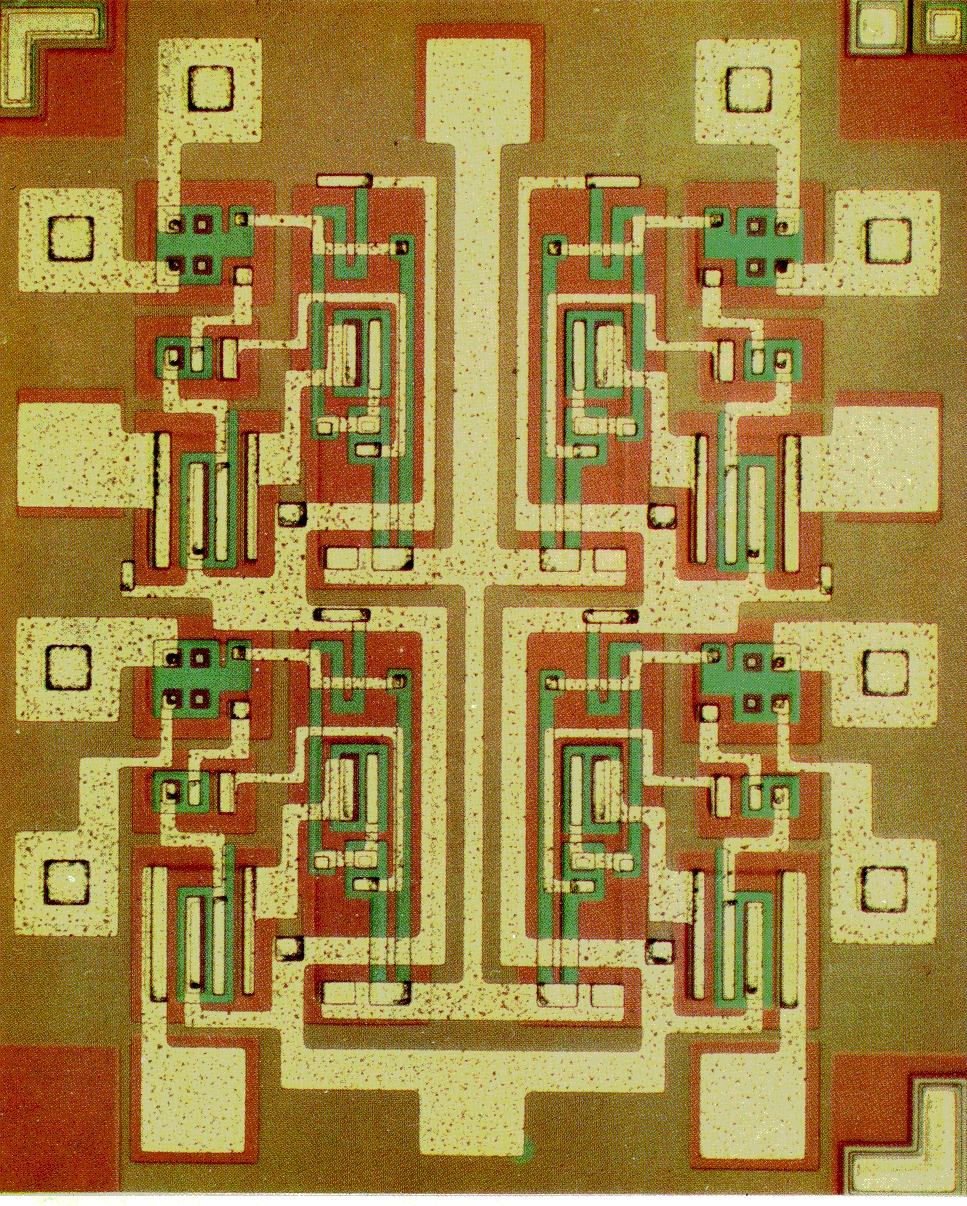
\includegraphics[width=0.8\textwidth]{img/4-fach-NAND-C10.jpg}
				\caption*{Hradla NAND.\footnote[frame]{Zdroj: \href{https://commons.wikimedia.org/wiki/File:4-fach-NAND-C10.JPG}{Dgarte/Commons}}}
			\end{figure}
		\end{column}
	\end{columns}
}

\frame{
	\frametitle{}
	\begin{figure}
		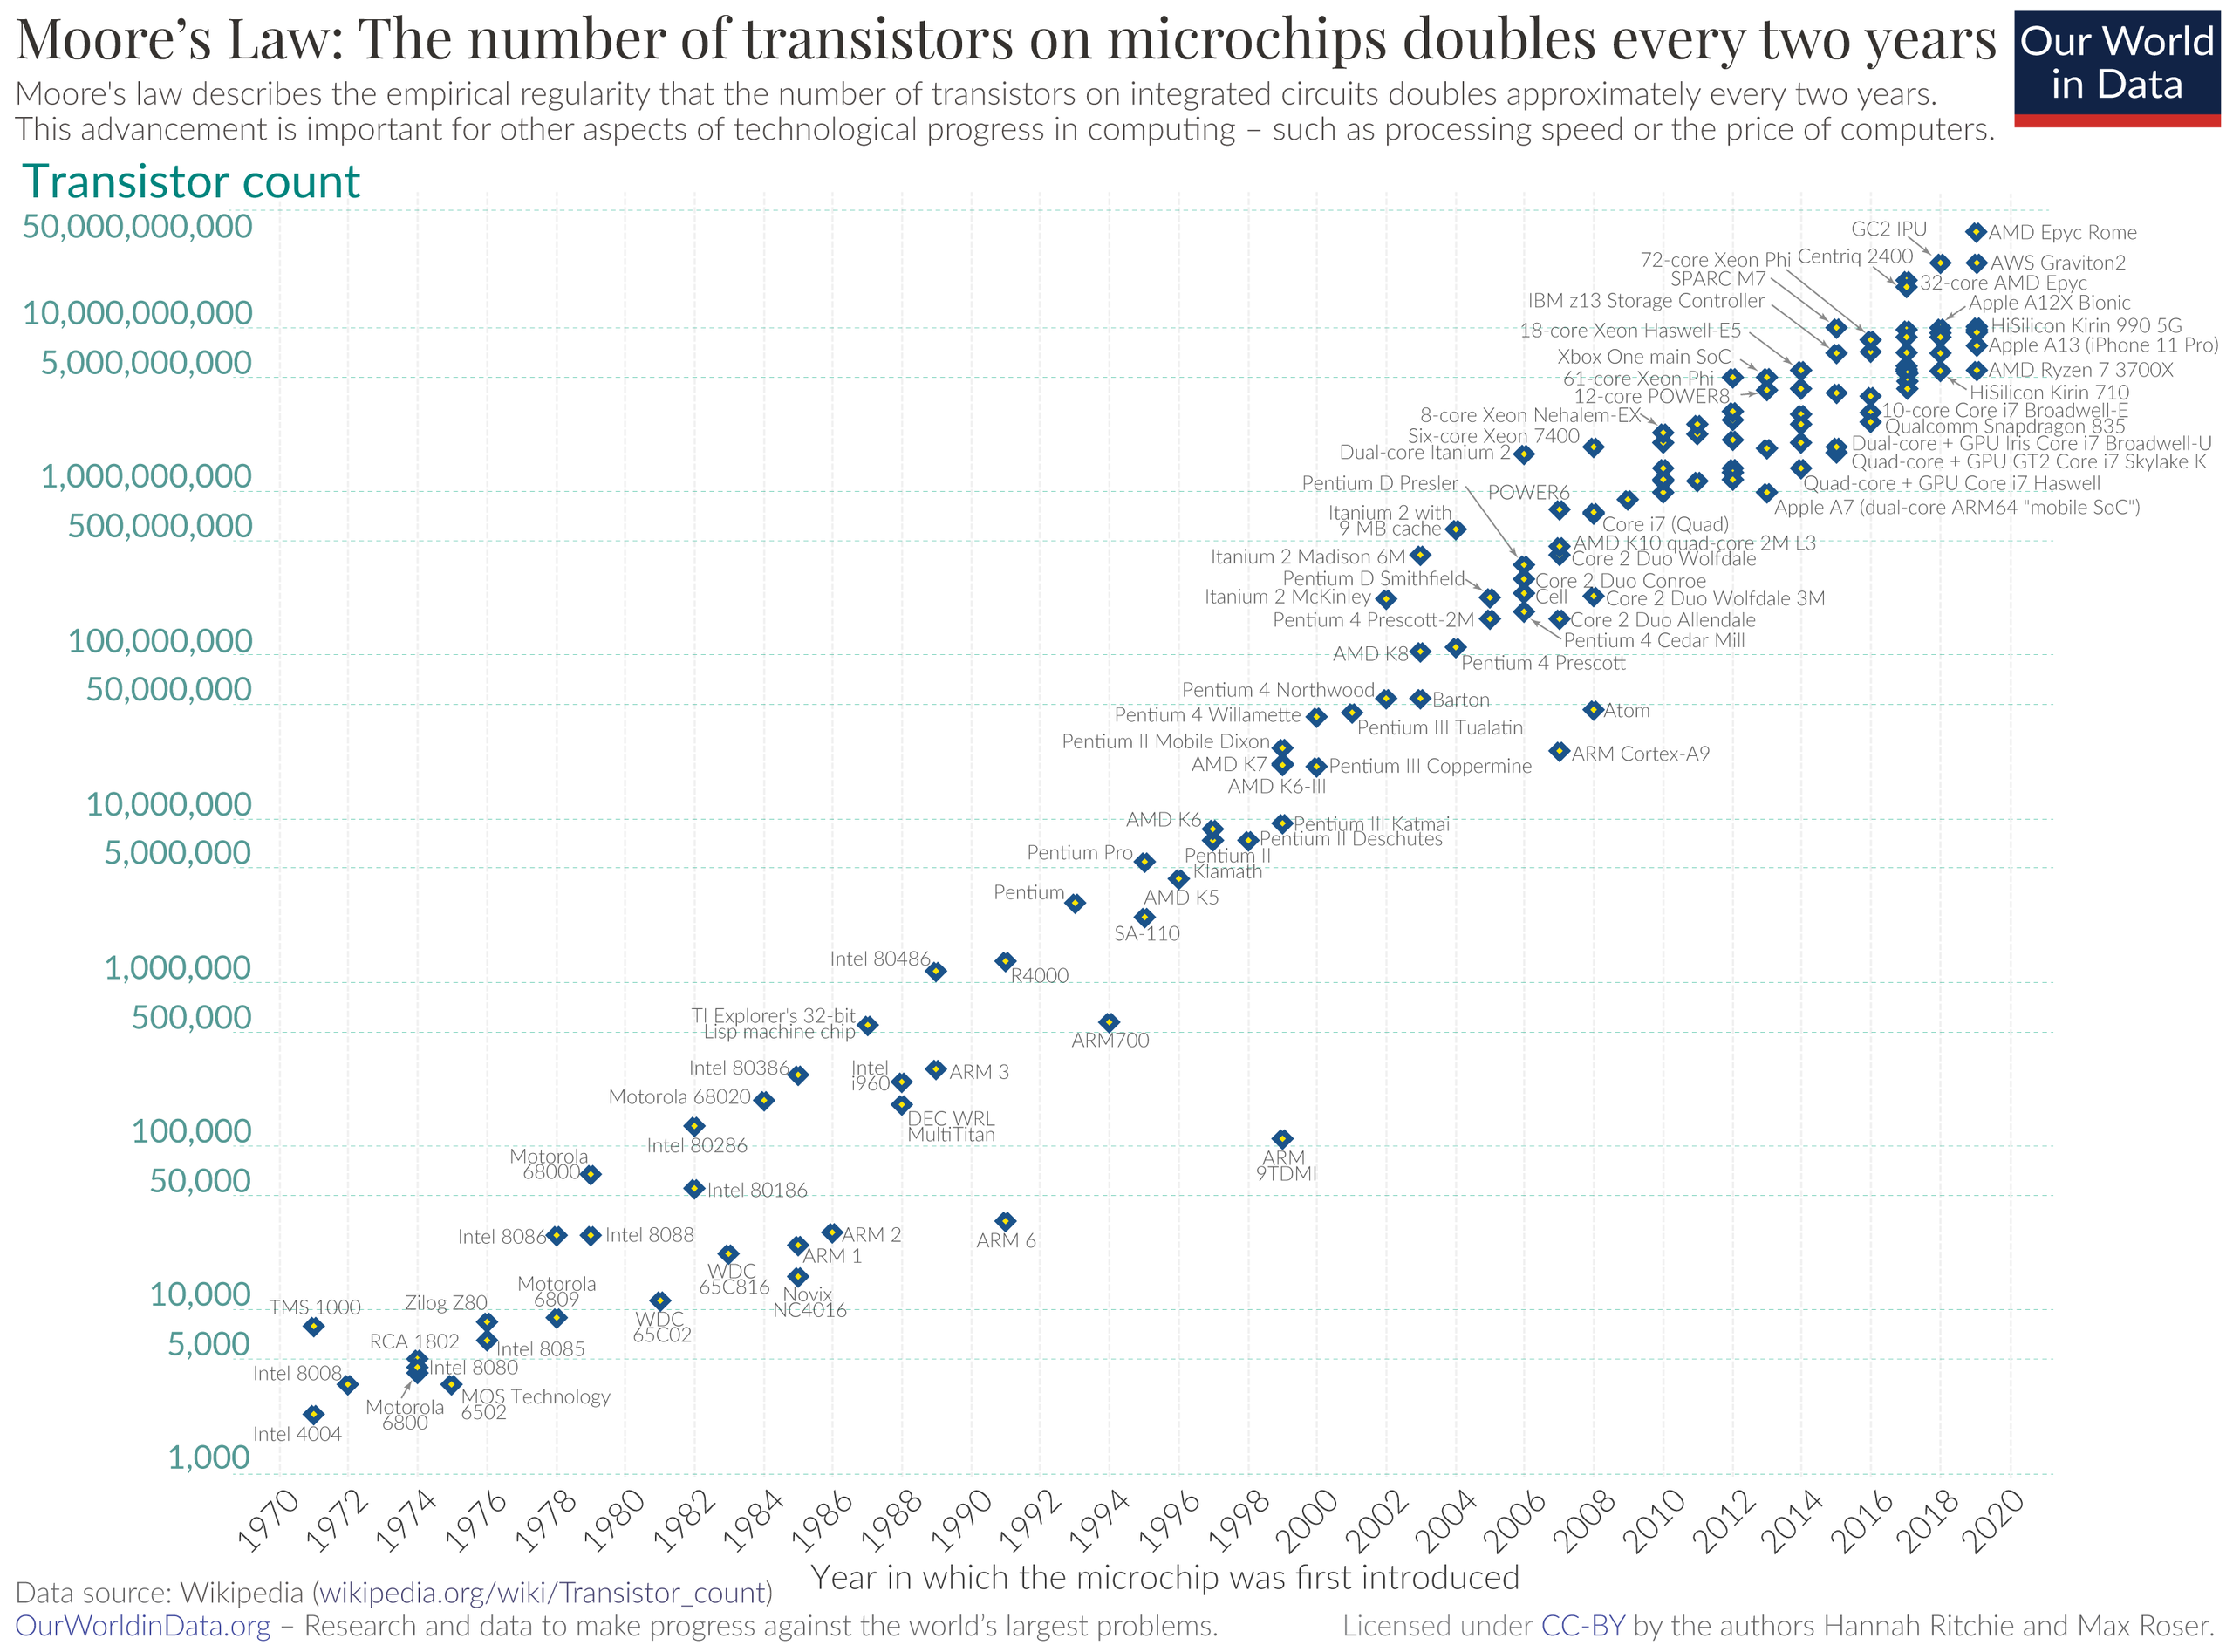
\includegraphics[width=0.8\textwidth]{img/Moores_Law_Transistor_Count_1970-2020.png}
		\caption*{Vývoj počtu tranzistorů na čipech v letech 1970--2020.\footnote[frame]{Zdroj: \href{https://en.wikipedia.org/wiki/File:Moore\%27s_Law_Transistor_Count_1970-2020.png}{Max Roser, Hannah Ritchie/Commons}}}
	\end{figure}
	\vfill
}

\subsection{Polovodičový průmysl v číslech}
\frame{
	\frametitle{}
	\begin{itemize}
		\item Celkové tržby
		\begin{itemize}
			\item 1987: \$33 000 000 000
			\item 1995: \$144 000 000 000
			\item 2000: \$204 000 000 000
			\item 2005: \$227 000 000 000
			\item 2010: \$298 320 000 000
			\item 2015: \$335 170 000 000
			\item 2018: \$481 090 000 000
		\end{itemize}
		\item Počet vyrobených integrovaných obvodů
		\begin{itemize}
			\item 1960--1996: 350 000 000 000
			\item 1997: 60 100 000 000
			\item 2005: 116 649 000 000
			\item 2010: 189 800 000 000
			\item 2015: 235 600 000 000
			\item 2018: 634 700 000 000
		\end{itemize}
	\end{itemize}
	\vfill
}

\frame{
	\frametitle{}
	\vfill
	\textbf{Silicon Valley}
	\begin{itemize}
		\item Jižní část San Francisco Bay v Severní Kalifornii.\footnote{\href{https://www.zive.cz/clanky/mapa-silicon-valley-kde-vlastne-lezi-legendarni-udoli/sc-3-a-157330/default.aspx}{Mapa Silicon Valley: kde vlastně leží legendární údolí?}}
		\item Dříve zde byly ovocné sady.
		\item V současnosti jde o světové centrum počítačového a technologického průmyslu, jsou zde převážně firmy vyvíjející křemíkové čipy a počítačovou techniku.
		\item Sídlí zde firmy Google, HP, Cisco, Intel, AMD, Adobe, Facebook, a další.
		\item Na téměř 5000 km$^2$ žije více než tři milióny lidí, z toho polovina je zde zaměstnána.\footnote{\href{https://siliconvalleyindicators.org/about/snapshot/}{Snapshot of the Region}}
	\end{itemize}
	\vfill
}

\frame{
	\frametitle{}
	\vfill
	\begin{figure}
		\adjincludegraphics[width=.9\textwidth]{img/Aerial_view_of_Silicon_Valley.jpg}
		\caption*{Letecký pohled na areál Silicon Valley.\footnote{\href{https://commons.wikimedia.org/wiki/File:Aerial_view_of_Silicon_Valley.jpg}{Zdroj: Patrick Nouhailler/Commons}}}
	\end{figure}
	\vfill
}

\section{Úvod -- germanium, cín, olovo a flerovium}
\frame{
	\frametitle{}
	\vfill
	\begin{tabular}{|c|l|l|l|}
	\hline
	 & \textit{Germanium} & \textit{Cín} & \textit{Olovo} \\\hline
	 El. konfigurace & 3d$^{10}$ 4s$^{2}$ 4p$^{2}$ & 4d$^{10}$ 5s$^{2}$ 5p$^{2}$ & 4f$^{14}$ 5d$^{10}$ 6s$^{2}$ 6p$^{2}$ \\\hline
	 Teplota tání [$^\circ$C] & 945 & 232 & 328 \\\hline
	 Teplota varu [$^\circ$C]  & 2850 & 2623 & 1749 \\\hline
	 Objeven & 1886 & cca 3500 př.n.l. & v 7. tis. př.n.l. \\\hline
	 Vzhled & bílostříbrný\footnote{Zdroj: \href{https://commons.wikimedia.org/wiki/File:Polycrystalline-germanium.jpg}{Jurii/Commons}} & bílostříbrný\footnote{Zdroj: \href{https://commons.wikimedia.org/wiki/File:Sn-Alpha-Beta.jpg}{Alchemist-hp/Commons}} & šedé\footnote{Zdroj: \href{https://commons.wikimedia.org/wiki/File:Lead_electrolytic_and_1cm3_cube.jpg}{Alchemist-hp/Commons}} \\
	 &  \begin{minipage}{.2\textwidth}
	 	\adjincludegraphics[width=\linewidth]{img/Polycrystalline-germanium.jpg}
	 \end{minipage}
	 	& \begin{minipage}{.2\textwidth}
	 		\adjincludegraphics[width=\linewidth]{img/Sn-Alpha-Beta.jpg}
	 	\end{minipage} & \begin{minipage}{.2\textwidth}
	 	\adjincludegraphics[width=\linewidth]{img/Lead_electrolytic_and_1cm3_cube.jpg}
 	\end{minipage} \\\hline
	\end{tabular}
	\vfill
}

\frame{
	\frametitle{}
	\vfill
	\textit{Flerovium}
		\begin{itemize}
			\item Umělý prvek, protonové číslo 114, Fl.
			\item Poprvé byl připraven v roce 1998:
			\item \ce{^{244}_{94}Pu + ^{48}_{20}Ca -> ^{292}_{114}Fl$^\star$ -> ^{290}_{114}Fl + 2 ^1_0n}
			\item Nejstabilnějším izotopem je $^{289}$Fl, T$_\frac{1}{2}$ = 1,9~s.
			\item \ce{^{289}_{114}Fl -> ^{285}_{112}Cn + $\alpha$}
			\item Prvek byl v roce 2011 pojmenován Flerovium na počest ruského fyzika Georgije Fljorova.\footnote[frame]{\href{https://old.iupac.org/publications/ci/2012/3404/iw1_periodic_table.html}{Flerovium and Livermorium Join the Periodic Table}}
	\end{itemize}

	\begin{figure}
		\adjincludegraphics[height=.3\textheight]{img/RUSMARKA-1660.jpg}
		\caption*{Georgij Fljorov.\footnote[frame]{\href{https://rusmarka.ru/files/sitedata/401/1439/e8f0957b-ec2e-4b01-99d1-42271fd3e506.jpg}{Zdroj: Rusmarka.net}}}
	\end{figure}
	\vfill
}

\section{Chemické a fyzikální vlastnosti}
\frame{
	\frametitle{}
	\vfill
	\begin{itemize}
		\item \textit{Germanium} je polokov s podobným měrným odporem jako křemík, ale s menší šířkou zakázaného pásu.
		\item Je elektropozitivnější a reaktivnější než křemík, rozpouští se v koncentrované kyselině sírové a dusičné.
		\item \textit{Cín} reaguje ochotně s chlorem a bromem i za nižší teploty.
		\item \textit{Olovo} v jemně práškovém stavu je pyroforické\footnote[frame]{Samozápalné}, ale v bulkovém stavu je poměrně málo reaktivní.
		\item Pasivuje se vrstvou nerozpustného produktu, např. \ce{PbSO4}.
		\item Prvky vytvářejí sloučeniny v oxidačních stavech II a IV. Stabilita stavu II roste v řadě Ge, Sn a Pb.
		\item Olovičité sloučeniny (např. \ce{PbO2}) jsou silná oxidační činidla.
		\item Podobně jako uhlík a křemík vytvářejí tyto prvky řetězce, ale s menší délkou.
	\end{itemize}
	\vfill
}

\frame{
	\frametitle{}
	\vfill
	\begin{itemize}
		\item \textit{Germanium} existuje ve dvou modifikacích, $\alpha$-Ge má kubickou krystalovou strukturu.
		\item Zvýšením tlaku (nad 12 GPa) dojde k přechodu na tetragonální formu $\beta$-Ge.\footnote[frame]{\href{https://doi.org/10.1016/j.jssc.2003.08.021}{Pressure-induced transformations in $\alpha$- and $\beta$-\ce{Ge3N4}: in situ studies by synchrotron X-ray diffraction}}
		\item \textit{Cín} existuje také ve dvou hlavních alotropních modifikacích.
		\item Za laboratorní teploty je stabilní tetragonální modifikace $\beta$-Sn.
		\item Při nízkých teplotách dochází k přechodu na kubickou modifikaci $\alpha$-Sn, která má diamantovou strukturu.
		\item K přechodu dochází pod teplotou 13,2~$^\circ$C.
		\item Změna modifikace (\ce{$\beta$ -> $\alpha$}) se označuje jako \textit{cínový mor}.\footnote[frame]{\href{https://www.youtube.com/watch?v=sXB83Heh3_c}{Transformation of beta tin into alpha modification}}
		\item Cínový mor je autokatalytický proces\footnote[frame]{Produkt urychluje reakci}, který způsobuje nevratné poškození cínových předmětů při nízkých teplotách.\footnote[frame]{\href{https://doi.org/10.1007/s11668-009-9280-8}{A Tin Pest Failure}}
		\item Za vysokých tlaků vznikají další dvě modifikace cínu $\delta$ a $\sigma$-Sn.
	\end{itemize}
	\vfill
}

\frame{
	\frametitle{}
	\vfill
	\begin{itemize}
		\item Olovo má díky vlivu inertního elektronové páru větší energetický rozdíl mezi valenčními s a p orbitaly.
		\item Proto netvoří kubickou (diamantovou) strukturu jako germanium a cín.
		\item Krystaluje v plošně centrované kubické struktuře tvořené ionty \ce{Pb^{2+}} spojenými kovovou vazbou.\footnote[frame]{\href{https://depts.washington.edu/matseed/mse_resources/Webpage/Metals/metalstructure.htm}{Structures of Metals}}
	\end{itemize}
	\begin{columns}
		\begin{column}{.5\textwidth}
			\begin{figure}
				\adjincludegraphics[height=.4\textheight]{img/Diamonds_glitter.png}
				\caption*{Struktura diamantu.\footnote[frame]{Zdroj: \href{https://commons.wikimedia.org/wiki/File:Diamonds_glitter.png}{ Anton/Commons}}}
			\end{figure}
		\end{column}
		\begin{column}{.5\textwidth}
	\begin{figure}
		\adjincludegraphics[height=.4\textheight]{img/Cubic-face-centered.png}
		\caption*{Plošně centrované kubická buňka.\footnote[frame]{Zdroj: \href{https://commons.wikimedia.org/wiki/File:Cubic-face-centered.svg}{Daniel Mayer, DrBob/Commons}}}
	\end{figure}
	\end{column}
	\end{columns}
	\vfill
}

\frame{
	\frametitle{}
	\vfill
	\textbf{Toxicita olova}
	\begin{itemize}
		\item Olovo je těžký kov, je toxický i v malých koncentracích a má jak akutní, tak i chronické účinky.\footnote[frame]{\href{https://dx.doi.org/10.1515/intox-2015-0009}{Lead toxicity: a review}}
		\item Toxické účinky lze vysvětlit vazbou olova na SH- skupiny enzymů, čímž dochází k jejich deaktivaci.\footnote[frame]{\href{http://web2.mendelu.cz/af_239_nanotech/J_Met_Nano/0314/pdf/jmn3-08.pdf}{Působení olova na živé organismy}}
		\item Toxicita olova je velkým problémem u dětí, u nichž může zpomalit duševní vývoj.\footnote[frame]{\href{https://www.sciencedaily.com/releases/2022/03/220307162011.htm}{Lead exposure in last century shrank IQ scores of half of Americans, study finds}}
		\item Typickými příznaky otravy olovem jsou bledost obličeje a rtů, nechutenství, anémie.
		\item Koncentrace olova v životním prostředí se stanovuje pomocí AAS, MS nebo diferenční pulzní voltametrie.
		\item Průmyslová spotřeba olova je průběžně snižována, využívají se bezolovnaté pájky, hledají se bezolovnaté náhrady střeliva.
	\end{itemize}
	\vfill
}

\section{Výskyt a získávání prvků}
\subsection{Germanium}
\frame{
	\frametitle{}
	\vfill
	\begin{itemize}
		\item Koncentrace germania v zemské kůře je okolo 1,6~ppm.\footnote[frame]{\href{https://doi.org/10.1016/j.oregeorev.2005.07.034}{Metallogenesis of germanium—A review}}
		\item Minerály germania jsou vzácné, jako hlavní zdroj slouží rudy zinku, mědi a olova.\footnote[frame]{\href{https://www.mindat.org/element/Germanium}{The mineralogy of Germanium}}
	\end{itemize}
	\begin{center}
	\begin{tabular}{|c|c|}
		\hline
		\textbf{Minerál} & \textbf{Složení} \\
		\hline
		Argutit &  \ce{GeO2} \\
		\hline
		Argyrodit & \ce{Ag8GeS6} \\
		\hline
		Bartelkeit & \ce{PbFeGe(Ge2O7)(OH)2 . H2O} \\
		\hline
		Briartit & \ce{Cu2(Zn,Fe)GeS4} \\
		\hline
		Germanit & \ce{Cu26Ge4Fe4S32} \\
		\hline
		Krieselit & \ce{Al2GeO4(OH)2} \\
		\hline
		Renierit & \ce{(Cu,Zn)11(Ge,As)2Fe4S16} \\
		\hline
	\end{tabular}
	\end{center}
	\vfill
}

\frame{
	\frametitle{}
	\vfill
	\begin{itemize}
		\item Germanium se primárně vyrábí z oxidu, ale v minerálech se nachází převážně ve formě sulfidu. Proto je prvním krokem pražení na vzduchu.
		\item \ce{GeS2 + 3 O2 -> GeO2 + 2 SO2}
		\item Pokud oxid obsahuje nečistoty, je možné ho vyčistit převedením na těkavý chlorid, který lze destilovat. Jde zvláště o zinek, který se chová velmi podobně jako germanium.\footnote[frame]{\href{https://doi.org/10.3103/S1067821207040049}{World market of germanium and its prospects}}
		\item \ce{GeO2 + 4 HCl -> GeCl4 + 2 H2O}
		\item \ce{GeO2 + 2 Cl2 -> GeCl4 + O2}
		\item Pro ocelářský průmysl se oxid redukuje uhlíkem.\footnote[frame]{\href{https://doi.org/10.1016/j.mineng.2003.11.014}{Review of germanium processing worldwide}}
		\item \ce{GeO2 + C -> Ge + CO2}
		\item Pro aplikace vyžadující vyšší čistotu, např. v polovodičovém průmyslu se redukuje vodíkem:
		\item \ce{GeO2 + 2 H2 -> Ge + 2 H2O}
	\end{itemize}

	\vfill
}

\subsection{Cín}
\frame{
	\frametitle{}
	\vfill
	\begin{columns}
		\begin{column}{.6\textwidth}
			\begin{itemize}
				\item Koncentrace cínu v zemské kůře je okolo 2,1~ppm.
				\item Hlavním minerálem cínu je \textit{cínovec} (\textit{kassiterir}, \ce{SnO2}).\footnote[frame]{\href{https://www.mindat.org/element/Tin}{The mineralogy of Tin}}
				\item Bronz, slitina mědi a cínu, byl znám a využíván už v pravěku a starověku, doba bronzová je datována do období 2300--800 let př. n. l. (v Evropě).
				\item Oblíbenost bronzu je dána třemi důvody:
				\begin{enumerate}
					\item Pro zpracování bronzu stačí nižší teploty než v případě železa (oceli).
					\item Jedná se o snadno dostupný kov.
					\item Dobré mechanické vlastnosti.
				\end{enumerate}
			\end{itemize}
		\end{column}
		\begin{column}{.4\textwidth}
			\begin{figure}
				\adjincludegraphics[width=.9\textwidth]{img/Pu_with_openwork_interlaced_dragons_design.jpg}
				\caption*{Bronzová nádoba.\footnote[frame]{Zdroj: \href{https://commons.wikimedia.org/wiki/File:Pu_with_openwork_interlaced_dragons_design.jpg}{Mountain/Commons}}}
			\end{figure}
		\end{column}
	\end{columns}
	\vfill
}

\frame{
	\frametitle{}
	\vfill
	\begin{itemize}
		\item \textbf{Kasiterit} (cínovec) je hlavním minerálem cínu. Je pojmenován po obci Cínovec v Krušných horách, v jejímž okolí byl těžen.
		\item Vzniká krystalizací z hydrotermálních vysokoteplotních roztoků, které jsou doprovodným jevem magmatické činnosti.
		\item Tvrdost 6-7, křehký.\footnote[frame]{\href{https://mineraly.sci.muni.cz/oxidy/kasiterit.html}{Atlas minerálů - kasiterit}}
	\end{itemize}
	\begin{columns}
		\begin{column}{.3\textwidth}
			\begin{figure}
				\adjincludegraphics[height=0.28\textheight]{img/Cassiterite-119419.jpg}
				\caption*{Cínovec z Bolívie.\footnote[frame]{Zdroj: \href{https://commons.wikimedia.org/wiki/File:Cassiterite-119419.jpg}{Robert M. Lavinsky/Commons}}}
			\end{figure}
		\end{column}

			\begin{column}{.3\textwidth}
			\begin{figure}
				\adjincludegraphics[height=0.28\textheight]{img/Cassiterite-jmix08-05a.jpg}
				\caption*{Cínovec z Číny.\footnote[frame]{Zdroj: \href{https://commons.wikimedia.org/wiki/File:Cassiterite-jmix08-05a.jpg}{Robert M. Lavinsky/Commons}}}
			\end{figure}
			\end{column}

			\begin{column}{.3\textwidth}
			\begin{figure}
				\adjincludegraphics[height=0.28\textheight]{img/Cinovec.jpg}
				\caption*{Obec Cínovec.\footnote[frame]{Zdroj: \href{https://commons.wikimedia.org/wiki/File:Zinnwald_(Erzgebirge)-Cinovec,_alter_Grenzübergang,_Ausreise.jpg}{Jens Jäpel/Commons}}}
			\end{figure}
		\end{column}
	\end{columns}
	\vfill
}

\frame{
	\frametitle{}
	\vfill
	\begin{itemize}
		\item Kasiterit lze snadno redukovat uhlíkem za vysoké teploty.
		\item Využívají se plamenné pece temperované na 1200--1300~$^\circ$C.
		\item Problém způsobuje železo přítomné v kasiteritu.
		\item Proto se redukce provádí postupně, nejprve se kasiterit praží na vzduchu, tím se zbaví síry, antimonu a arsenu.
		\item Potom se vylouhuje v kyselině za vysoké teploty a následně se redukuje uhlím v peci.
		\item \ce{SnO2 + CO -> SnO + CO2}
		\item \ce{SnO + CO -> Sn + CO2}
		\item Během redukce vzniká velké množství strusky, která obsahuje křemičitan cínatý, proto se i struska dále redukuje buď koksem nebo železným odpadem.
		\item \ce{SnSiO3 + CaO + C -> Sn + CaSiO3 + CO}
		\item \ce{SnSiO3 + Fe -> Sn + FeSiO3}
	\end{itemize}
	\vfill
}

\frame{
	\frametitle{}
	\vfill
	\begin{figure}
		\adjincludegraphics[height=.7\textheight]{img/SnPrice.png}
		\caption*{Vývoj ceny a produkce cínu.\footnote[frame]{Zdroj: \href{https://commons.wikimedia.org/wiki/File:SnPrice.png}{Materialscientist/Commons}}}
	\end{figure}
	\vfill
}

\subsection{Olovo}
\frame{
	\frametitle{}
	\vfill
	\begin{itemize}
		\item Koncentrace olova v zemské kůře je okolo 16~ppm.
		\item V mořské vodě je jeho obsah jen 0,03~mg.kg$^{-1}$.
		\item Tři ze čtyř přirozených izotopů olova (\ce{^{206}Pb, ^{207}Pb a ^{208}Pb}) jsou posledním, stabilním produktem rozpadových řad uranu a thoria.
		\item Nevyskytuje se v čisté stavu, ale je součástí mnoha minerálů.\footnote[frame]{\href{https://www.mindat.org/element/Lead}{The mineralogy of Lead}} Nejdůležitější je \textit{galenit} (PbS), který slouží jako zdroj pro průmyslovou výrobu.
	\end{itemize}
	\begin{center}
		\begin{tabular}{|c|c|}
			\hline
			galenit & \ce{PbS} \\\hline
			anglesit &  \ce{PbSO4} \\\hline
			cerussit &  \ce{PbCO3} \\\hline
			pyromorfit &  \ce{Pb5(PO4)3Cl} \\\hline
			cerussit &  \ce{Pb5(AsO4)3Cl} \\\hline
		\end{tabular}
	\end{center}
	\vfill
}

\frame{
	\frametitle{}
	\vfill
	\begin{figure}
		\adjincludegraphics[width=\textwidth]{img/Radioactive_decay_chains_diagram.png}
		\caption*{Rozpadové řady.\footnote[frame]{Zdroj: \href{https://commons.wikimedia.org/wiki/File:Radioactive_decay_chains_diagram.svg}{Johantheghost/Commons}}}
	\end{figure}
	\vfill
}

\frame{
	\frametitle{}
	\vfill
	\textbf{Galenit}
	\begin{itemize}
		\item Sulfid olovnatý, PbS, dříve byl označován jako \textit{olověné blejno}.\footnote[frame]{\href{http://www.rimbaba.cz/index.php/mineralogie/31-lestenec-pbs}{Galenit (leštěnec olověný, blejno olověné) - PbS}}
		\item Krystalová struktura odpovídá typu NaCl.\footnote[frame]{\href{http://mineraly.sci.muni.cz/sulfidy/galenit.html}{Atlas minerálů - galenit}}$^,$\footnote[frame]{\href{http://mineralogie.sci.muni.cz/kap_7_4_sulfid/kap_7_4_sulfidy.htm\#7.4.2.1.}{Systematická mineralogie - galenit}}
		\item Je to jeden z nejrozšířenějších sulfidových minerálů.
		\item Ve struktuře pravidla obsahuje další prvky, např. Bi, Cd, As a Te.
		\item V Česku ho nacházíme ve Stříbře a Příbrami, těžba probíhala v Harrachově.
		\item Ve Starověkém Egyptě galenit nahradil malachitový prášek (\ce{Cu2(OH)2CO3}), který sloužil k výrobě zeleného líčidla na oči (tehdy nezbytnou součástí každodenního života egyptských žen i mužů). S galenitem se stalo módní líčení černých linek.
	\end{itemize}
	\vfill
}

\frame{
	\frametitle{}
	\vfill
	\begin{columns}
		\begin{column}{.45\textwidth}
			\begin{figure}
				\adjincludegraphics[height=0.45\textheight]{img/Fluorite-Galena-flu35c.jpg}
				\caption*{Galenit, PbS.\footnote[frame]{Zdroj: \href{https://commons.wikimedia.org/wiki/File:Fluorite-Galena-flu35c.jpg}{Robert M. Lavinsky/Commons}}}
			\end{figure}
		\end{column}

		\begin{column}{.45\textwidth}
			\begin{figure}
				\adjincludegraphics[height=0.45\textheight]{img/NaCl_polyhedra.png}
				\caption*{Struktura NaCl.\footnote[frame]{Zdroj: \href{https://commons.wikimedia.org/wiki/File:NaCl_polyhedra.svg}{Goran tek-en/Commons}}}
			\end{figure}
		\end{column}
	\end{columns}
	\vfill
}

\frame{
	\frametitle{}
	\vfill
	\textbf{Cerusit}
	\begin{itemize}
		\item Uhličitan olovnatý, \ce{PbCO3}.\footnote[frame]{\href{https://www.mindat.org/min-934.html}{Cerussite}}
		\item Krystaluje v orthorombické soustavě.\footnote[frame]{\href{https://mineraly.sci.muni.cz/karbonaty/cerusit.html}{Atlas minerálů - cerusit}}
		\item Často vzniká oxidací galenitu a dalších nerostů olova.
		\item V Česku ho nacházíme ve Stříbře, velké krystaly pocházejí z Namibie.
	\end{itemize}

	\begin{columns}
		\begin{column}{.4\textwidth}
			\begin{figure}
				\adjincludegraphics[width=0.7\textwidth]{img/Cerussite-18566.jpg}
				\caption*{Cerusit z Namíbie.\footnote[frame]{Zdroj: \href{https://commons.wikimedia.org/wiki/File:Cerussite-18566.jpg}{Robert M. Lavinsky/Commons}}}
			\end{figure}
		\end{column}

		\begin{column}{.4\textwidth}
			\begin{figure}
				\adjincludegraphics[width=0.7\textwidth]{img/Cerussite-Malachite-Mimetite-158529.jpg}
				\caption*{Cerusite, malachit a mimetit.\footnote[frame]{Zdroj: \href{https://commons.wikimedia.org/wiki/File:Cerussite-Malachite-Mimetite-158529.jpg}{Robert M. Lavinsky/Commons}}}
			\end{figure}
		\end{column}
	\end{columns}
	\vfill
}

\frame{
	\frametitle{}
	\vfill
	\begin{itemize}
		\item Olovo se připravuje nejčastěji oxidací galenitu a následnou redukcí vzniklého oxidu.
		\item \ce{2 PbS + 3 O2 -> 2 PbO + SO2}
		\item \ce{PbO + C -> Pb + CO}
		\item \ce{PbO + CO -> Pb + CO2}
		\item Redukci uhlíkem lze nahradit redukcí galenitem.
		\item \ce{2 PbO + PbS -> 3 Pb + SO2}
	\end{itemize}
	\begin{figure}
		\adjincludegraphics[width=0.4\textwidth]{img/Metaloyrgiagalikis.jpg}
		\caption*{Pec na výrobu olova.\footnote[frame]{Zdroj: \href{https://commons.wikimedia.org/wiki/File:Metaloyrgiagalikis.jpg}{Dr Peter Tzeferis/Commons}}}
	\end{figure}
	\vfill
}

\frame{
	\frametitle{}
	\vfill
	\textbf{Recyklace olova}
	\begin{itemize}
		\item Důležitým zdrojem olova (ale i jiných kovů) je recyklace.\footnote[frame]{\href{https://www.youtube.com/watch?v=eO-X8Gw2nXY}{Lead Battery Recycling Process}}
		\item Většina současné produkce olova je využita pro konstrukci olověných akumulátorů, proto se hledají cesty k jejich recyklaci.\footnote[frame]{\href{https://doi.org/10.1016/j.resconrec.2018.09.012}{Sustainability evaluation of secondary lead production from spent lead acid batteries recycling}}
		\item Recyklují se nejen olověné elektrody, ale i plastový obal a elektrolyt.
		\item V roce 2014 byly v užívání akumulátory o celkové kapacitě 429~GWh.
		\item Recyklaci lze popsat rovnicemi:
	\end{itemize}
	\begin{align*}
		\ce{PbSO4 + Na2CO3 &-> PbO + Na2SO4 + CO2}\\
		\ce{PbO + C &-> 2 Pb + CO2}\\
		\ce{PbSO4 + 2 C &-> PbS + CO2}\\
		\ce{PbS + Fe &-> Pb + FeS}\\
	\end{align*}
	\vfill
}

\section{Využití prvků}
\subsection{Germanium -- polovodičová technika}
\frame{
	\frametitle{}
	\vfill
	\begin{itemize}
		\item Germanium je polovodič s menší šířkou zakázaného pásu než má křemík.
		\item Hlavní využití v polovodičovém průmyslu nachází ve \textit{fotovoltaických panelech}.\footnote[frame]{\href{https://www.pv-magazine.com/2021/01/15/germanium-based-solar-cell-tech-for-agrivoltaics/}{Germanium-based solar cell tech for agrivoltaics}}
		\item Díky podobným mřížkovým parametrům je možné germanium využít jako substrát pro depozici vrstev \ce{GaAs}.
		\item Slitina křemíku s germaniem se používá jako polovodič v integrovaných obvodech pro vysoké frekvence a má také termoelektrické vlastnosti.
	\end{itemize}
	\begin{figure}
		\adjincludegraphics[height=.45\textheight,angle=90]{img/MidSTAR-1.jpg}
		\caption*{Satelit MidSTAR-1.\footnote[frame]{Zdroj: \href{https://commons.wikimedia.org/wiki/File:MidSTAR-1.jpg}{United States Naval Academy/Commons}}}
	\end{figure}
	\vfill
}

\subsection{Germanium -- optika}
\frame{
	\frametitle{}
	\vfill
	\begin{itemize}
		\item Germanium má vysoký index lomu (4,0) a velmi dobrou prostupnost v infračervené oblasti spektra, proto se využívá např. při konstrukci krystalů pro FTIR-ATR spektrometry,\footnote[frame]{\href{https://specac.com/choosing-the-right-atr-crystal/}{Choosing the right ATR crystal}} infračervené senzory a přístroje na noční vidění.
		\item Oxid germaničitý (\ce{GeO2}) se využívá v optických vláknech a čočkách širokoúhlých kamer.
		\item GST (\ce{GeSbTe}) - ternární slitina, využívá se v přepisovatelných DVD médiích a také ve speciálních typech pamětí využívajících přechod mezi nevodivou amorfní a polovodivou krystalickou formou.
	\end{itemize}
	\begin{figure}
		\adjincludegraphics[width=.8\textwidth]{img/ATR_path-en.png}
		\caption*{Princip FTIR-ATR.\footnote[frame]{Zdroj: \href{https://commons.wikimedia.org/wiki/File:ATR_path-en.svg}{Fulvio314/Commons}}}
	\end{figure}
	\vfill
}

\subsection{Germanium -- katalyzátor}
\frame{
	\frametitle{}
	\vfill
	\begin{itemize}
		\item Oxid germaničitý se využívá (převážně v Japonsku) jako katalyzátor při výrobě polyesterů, např. PET, polykondenzačními reakcemi.\footnote[frame]{\href{https://doi.org/10.1080/00914030108035115}{The Current Status of Catalysis and Catalyst Development for the Industrial Process of Poly(ethylene terephthalate) Polycondensation}}
		\item Alternativou jsou katalyzátory na bázi antimonu nebo titanu.
	\end{itemize}
	\begin{figure}
		\adjincludegraphics[width=0.85\textwidth]{img/Polyethyleneterephthalate.png}
	\end{figure}
	\vfill
}

\subsection{Cín -- slitiny}
\frame{
	\frametitle{}
	\begin{columns}
		\begin{column}{.7\textwidth}
			\begin{itemize}
				\item Kovový cín nemá příliš dobré mechanické vlastnosti, proto se potkáváme zpravidla s jeho slitinami.
				\item Velmi důležité jsou \textbf{pájky}, slitiny cínu s olovem. Obsah cínu je v rozmezí 2--63~\%, typicky 33~\%. Často se přidává další kov pro lepší tavitelnost (Cd, Ga, In nebo Bi).
				\item \textit{Tvrdé pájky} -- tají nad teplotou 450~$^\circ$C, obvykle slitina cínu s mědí, zinkem a stříbrem nebo slitiny hliníku.
				\item \textit{Měkké pájky} -- tají pod teplotou 450~$^\circ$C, slitiny cínu s olovem.
				\item \textit{Bezolovnaté pájky} -- prosazovány z ekologických důvodů, ale jejich vlastnosti jsou zatím horší, než vlastnosti klasických pájek.
			\end{itemize}
		\end{column}

		\begin{column}{.35\textwidth}
			\begin{figure}
				\adjincludegraphics[width=\textwidth]{img/Soldering-PCB-b.jpg}
				\caption*{Deska s plošnými spoji.\footnote[frame]{Zdroj: \href{https://commons.wikimedia.org/wiki/File:Soldering-PCB-b.jpg}{Tlapicka/Commons}}}
			\end{figure}

			\begin{itemize}
				\item \textit{SAC} -- slitiny cínu, stříbra a/nebo mědi (Sn/Ag/Cu).
				\item Teploty tání okolo 220 °C.
			\end{itemize}
		\end{column}
	\end{columns}
	\vfill
}

\subsubsection{Nízkotající slitiny}
\frame{
	\frametitle{}
	\textbf{Nízkotající slitiny}
	\begin{tabular}{|l|l|l|}
		\hline
		\textbf{Slitina} & \textbf{Obchodní název} & \textbf{Teplota tání [$^\circ$C]} \\
		\hline
		\textbf{Bi45Pb23Sn8In19Cd5} & Slitina 47  &  47 \\
		\hline
		\textbf{Bi49Pb18Sn12In21} & Slitina 58  & 58 \\
		\hline
		\textbf{Bi50Pb27Sn13Cd} & Woodův kov 1 & 68-72 \\
		\hline
		\textbf{Bi50Pb25Sn12Cd} & Woodův kov 2 & 60-64 \\
		\hline
		\textbf{Bi50Sn25Pb} & Roseův kov & 92-96 \\
		\hline
		\textbf{Bi55Pb32Sn} & Molotův kov & 96-98 \\
		\hline
		\textbf{Bi74Pb7Sn} & Biola 1 & 104-463 \\
		\hline
		\textbf{Bi50Pb43Cd} & Biola 3 & 80-84 \\
		\hline
		\textbf{Bi8Sn57Pb} & Stabia 1 & 139-178 \\
		\hline
		\textbf{Pb45Bi10Sn} & Stabia 4 & 97-169 \\
		\hline
		\textbf{Pb25Bi25Sn} & Stabia 6 & 97-161 \\
		\hline
		\textbf{Pb73Bi23Sn3Zn} & Plumbia 3 & 183-224 \\
		\hline
		\textbf{Pb57Bi8Sn} & Plumbia 5 & 174-214 \\
		\hline
	\end{tabular}
}

\subsection{Pocínované plechy}
\frame{
	\frametitle{}
	\begin{columns}
		\begin{column}{.75\textwidth}
			\begin{itemize}
				\item Téměř polovina produkce cínu se používá pro povrchovou úpravu kovů -- \textit{pocínování}.
				\item Vrstva cínu je netoxická a chrání kov před korozí.
				\item Její tloušťka je od 0,4 do 25 $\mu$m.
				\item Cínování se provádí buď galvanickým pokovováním (roztoky solí cínu v methansulfonové kyselině, \ce{CH3SO3H}) nebo ponořením předmětu do taveniny cínu.
				\item Pocínované plechy se využívají v potravinářství. Plechovky na potraviny jsou z běžných ocelových materiálů, vnitřní strana je pocínovaná, aby nedocházelo ke kontaminaci potravin.\footnote[frame]{\href{http://www.povrchove-technologie.cz/cz/technologie/cinovani-matne--leskle/}{Cínování matné / lesklé}}
			\end{itemize}
		\end{column}

		\begin{column}{.3\textwidth}
			\begin{figure}
				\adjincludegraphics[width=\textwidth]{img/Weissblech_verpackungsstahl.jpg}
				\caption*{Pocínované plechy.\footnote[frame]{Zdroj: \href{https://commons.wikimedia.org/wiki/File:Weissblech_verpackungsstahl.jpg}{ThyssenKrupp Rasselstein GmbH/Commons}}}
			\end{figure}

			\begin{figure}
				\adjincludegraphics[width=.7\textwidth]{img/CH3SO3H.png}
				\caption*{Kyselina methansulfonová.}
			\end{figure}
		\end{column}
	\end{columns}
	\vfill
}

\subsection{Cín -- ITO}
\frame{
	\frametitle{}
	\begin{itemize}
		\item Směs oxidů inditého a cíničitého, přibližný vzorec je \ce{(In2O3)0_{.9} . (SnO2)_{0.1}}
		\item Je to nejrozšířenější transparentní a vodivý oxid.
		\item Lze z něj snadno připravit tenký, vodivý film.\footnote[frame]{\href{https://www.researchgate.net/publication/321172668_Structural_Optical_and_Electrical_Properties_of_ITO_Thin_Films}{Structural, Optical and Electrical Properties of ITO Thin Films}}
		\item Poměr transparentnosti a vodivosti filmu lze řídit tloušťkou filmu.
		\begin{itemize}
			\item Tenký film je vysoce průhledný, ale má vyšší odpor.
			\item Silnější vrstvy jsou méně průhledné, ale mají nižší elektrický odpor.
		\end{itemize}
		\item Lze vyrobit vysoce průhledný film s dostatečným elektrickým odporem, např. pro odledování oken letadel.\footnote[frame]{\href{https://phys.org/news/2019-08-defrosting-surfaces-seconds.html}{Defrosting surfaces in seconds}}
	\end{itemize}
	\vfill
}

\frame{
	\frametitle{}
	\vfill
	\begin{columns}
		\begin{column}{.5\textwidth}
			\begin{figure}
				\adjincludegraphics[height=.55\textheight]{img/Kristallstruktur_Lanthanoid-C-Typ.png}
				\caption*{Krystalová struktura ITO.\footnote[frame]{Zdroj: \href{https://commons.wikimedia.org/wiki/File:Kristallstruktur_Lanthanoid-C-Typ.png}{Orci/Commons}}}
			\end{figure}
		\end{column}
		\begin{column}{.5\textwidth}
			\begin{figure}
				\adjincludegraphics[height=.55\textheight]{img/lossy-page1-834px-ITO_grains_on_glass.jpg}
				\caption*{Snímek filmu z ITO.\footnote[frame]{Zdroj: \href{https://commons.wikimedia.org/wiki/File:ITO_grains_on_glass.tif}{Topliuchao/Commons}}}
			\end{figure}
		\end{column}
	\end{columns}
	\vfill
}

\subsection{Cín -- Katalýza}
\frame{
	\frametitle{}
	\begin{itemize}
		\item Oxidy cínu se využívají jako \textit{heterogenní katalyzátory}, např. směsné oxidy Sn-V se používají pro oxidaci benzenu a toluenu.
		\item Chlorid cíničitý lze použít ke katalýze Friedel-Craftsových alkylací, acylací a cyklizací.\footnote[frame]{\href{https://www.sciencedirect.com/topics/chemistry/intramolecular-friedel-crafts-acylation}{The Formation of Cyclic Ketones}}
	\end{itemize}
	\begin{center}
		\adjincludegraphics[width=0.7\textwidth]{img/SnCl4-FriedelCrafts.png}
	\end{center}
	\begin{itemize}
	\item Chlorid cíničitý se také používá na tvrzení skleněných lahví.
	\item Na povrchu skla se vytvoří tenká, transparentní vrstva \ce{SnO2}, která zvyšuje mechanickou odolnost skla.
	\end{itemize}
	\vfill
}

\subsection{Olovo -- Stínění radioaktivity}
\frame{
	\frametitle{}
	\begin{itemize}
		\item Díky vysoké atomové hmotnosti (velkému počtu elektronů) a malému atomovému poloměru dokáže olovo účinně stínit ionizující a RTG záření.\footnote[frame]{\href{https://www.worldcat.org/title/structural-shielding-design-for-medical-x-ray-imaging-facilities/oclc/1058579305}{Structural shielding design for medical X-ray imaging facilities)}}
		\item Toho se využívá v RTG technice, jaderných elektrárnách, radiochemických laboratořích, armádě, atd.
	\end{itemize}
	\begin{center}
		\adjincludegraphics[height=.45\textheight]{img/PB231460.JPG}
		\adjincludegraphics[height=.45\textheight]{img/PB271494.JPG}
	\end{center}
	\vfill
}

\subsection{Olověné akumulátory}
\frame{
	\frametitle{}
	\begin{columns}
		\begin{column}{.7\textwidth}
			\begin{itemize}
				\item Vynalezeny roku 1859 francouzským fyzikem Gastonem Planté.\footnote[frame]{\href{https://web.archive.org/web/20150929011427/http://lead-acid.com/lead-acid-battery-history.shtml}{Lead Acid Battery history}}$^,$\footnote[frame]{\href{http://www.corrosion-doctors.org/Biographies/PlantelBio.htm}{Gaston Planté (1834-1889)}}
				\item Jsou tvořeny olověnými elektrodami, jako elektrolyt slouží kyselina sírová.
				\item Oproti jiným typům baterií dokáží krátkodobě dodávat i velmi vysoký proud ($>$100~A).
				\item Vyrábějí se v kapacitách od 1~Ah do 10~kAh.\footnote[frame]{\href{https://www.pveducation.org/pvcdrom/battery-characteristics/battery-capacity}{Battery Capacity}}
				\item Využívají se pro startování automobilů, jako záložní zdroje, atd.
			\end{itemize}
		\end{column}

		\begin{column}{.25\textwidth}
			\begin{figure}
				\adjincludegraphics[height=.22\textheight]{img/Photo-CarBattery.jpg}
				\caption*{Autobaterie.\footnote[frame]{Zdroj: \href{https://commons.wikimedia.org/wiki/File:Photo-CarBattery.jpg}{Shaddack/Commons}}}

				\adjincludegraphics[height=.22\textheight]{img/Car_battery_cross-section.jpg}
				\caption*{Řez autobaterií.\footnote[frame]{Zdroj: \href{https://commons.wikimedia.org/wiki/File:Car_battery_cross-section.jpeg}{Ben Cossalter/Commons}}}
			\end{figure}
		\end{column}
	\end{columns}

	\vfill
}

\frame{
	\frametitle{}
	\begin{itemize}
		\item Nabitá baterie má kladnou elektrodu z oxidu olovičitého a zápornou z olova.
		\item Vybitá baterie má obě elektrody tvořené síranem olovnatým.
		\item Vybíjení:
		\item \ce{Pb + PbO2 + 2 H2SO4 -> 2 PbSO4 + 2 H2O}
		\item Nabíjení:
		\item \ce{2 PbSO4 + 2 H2O -> Pb + PbO2 + 2 H2SO4}
	\end{itemize}
	\begin{figure}
		\adjincludegraphics[height=.2\textheight]{img/OlovenyAkumulator.png}
	\end{figure}
	\vfill
}

\subsection{Olovo -- pigmenty}
\frame{
	\frametitle{}
	\begin{itemize}
		\item Olovo je součástí několika pigmentů, vzhledem k toxicitě olova se ale už dnes nepoužívají.
		\item Chromová žluť, \ce{PbCrO4}, v přírodě se nachází jako minerál \textit{krokoit}.\footnote[frame]{\href{https://mineraly.sci.muni.cz/sulfaty/krokoit.html}{Krokoit}} Má silné oxidační účinky.\footnote[frame]{\href{https://pubchem.ncbi.nlm.nih.gov/compound/24460}{Lead chromate -- PubChem}}
		\item Minium neboli olověná červeň, \ce{Pb3O4}, dnes se v menší míře používá při barvení skla. Dříve byl základní barvou nátěrových hmot pro železné konstrukce.
		\item Olověná běloba, \ce{PbCO3}, dříve se používala jako základová barva v nátěrech na dřevo, dnes se už používá minimálně.
		\begin{itemize}
			\item Reakcí se sulfanem ve vzduchu dochází k černání, vzniká sulfid olovnatý.
			\item \ce{PbCO3 + H2S -> PbS + CO2 + H2O}
		\end{itemize}
	\end{itemize}
	\vfill
}

\frame{
	\frametitle{}
	\vfill
	\begin{tabular}{ccc}
		\adjincludegraphics[height=.35\textheight]{img/Lead_chromate.jpg} &
		\adjincludegraphics[height=.35\textheight]{img/Red_lead.jpg} &
		\adjincludegraphics[height=.35\textheight]{img/BleiweissDuerer.jpg} \\
		Chromová žluť, \ce{PbCrO4}.\footnote[frame]{Zdroj: \href{https://commons.wikimedia.org/wiki/File:Lead_chromate.JPG}{FK1954/Commons}}
		&
		Minium, \ce{Pb3O4}.\footnote[frame]{Zdroj: \href{https://commons.wikimedia.org/wiki/File:Red_lead.jpg}{BXXXD/Commons}}
		&
		Olověná běloba, \ce{PbCO3}.\footnote[frame]{Zdroj: \href{https://commons.wikimedia.org/wiki/File:BleiweissDuerer.JPG}{Concord/Commons}}
	\end{tabular}
	\vfill
}

\section{Sloučeniny}
\subsection{Hydridy}
\frame{
	\frametitle{}
	\vfill
	\begin{itemize}
		\item \textbf{Germany} jsou skupinou hydridů s obecným vzorcem \ce{Ge$_n$H$_{2n+2}$} pro n = 1--5.
		\item Jsou to plyny nebo těkavé kapaliny, vlastnosti mají podobné jako silany.
	\end{itemize}

	\begin{tabular}{|l|r@{,}l|l|r@{,}l|l|l|}
	\hline
	& \multicolumn{2}{|c|}{\ce{GeH4}} & \ce{Ge2H6} & \multicolumn{2}{|c|}{\ce{Ge3H8}}
	& \ce{Ge4H10} & \ce{Ge5H12} \\\hline
	Teplota tání [$^\circ$C] & $-$164 & 8 & $-$109 & $-$105 & 6 & - & - \\\hline
	Teplota varu [$^\circ$C] & $-$88 & 1 & 29 & 110 & 5 & 176,9 & 234 \\\hline
	\end{tabular}

	\begin{itemize}
		\item \textbf{Halogengermany}, \ce{GeH_xX_{4-x}}, jsou bezbarvé, těkavé, reaktivní kapaliny
		\item Připravují se reakcí Ge, \ce{GeX2}, \ce{GeH2X2} nebo \ce{GeH4} s halogenvodíky.\footnote[frame]{\href{https://doi.org/10.1016/0020-1650(71)80119-8}{Mixed halogenomonogermanes}}
		\item \ce{GeH2Cl2 + 2 HI -> GeH2I2 + 2 HCl}
	\end{itemize}
}

\frame{
	\frametitle{}
	\vfill
	\begin{itemize}
		\item \textbf{German} (\ce{GeH4}) byl detekován v atmosféře Jupiteru.\footnote[frame]{\href{https://dx.doi.org/10.1086/160516}{The tropospheric gas composition of Jupiter's north equatorial belt /NH3, PH3, CH3D, GeH4, H2O/ and the Jovian D/H isotopic ratio}}
		\item Lze jej připravit rozkladem germanidů kovů, např. \ce{Mg2Ge}, kyselinou chlorovodíkovou.
		\item \ce{Mg2Ge + 4 HCl -> GeH4 + 2 MgCl2}
		\item Nereaguje s vodnými roztoky kyselin.
		\item V kapalném amoniaku se chová jako kyselina:
		\item \ce{GeH4 + NH3 <=> GeH3- + NH4+}
		\item Při reakci s alkalickými kovy v kapalném amoniaku dochází k redukci a uvolnění vodíku.
		\item \ce{2 K + 2 GeH4 ->[NH3 (l)] 2 KGeH3 + H2}
	\end{itemize}
	\vfill
}

\frame{
	\frametitle{}
	\vfill
	\begin{itemize}
		\item \textbf{Digerman}, \ce{Ge2H6}, je bezbarvá kapalina (T$_v$ = 29~$^\circ$C, T$_t$ = $-$109~$^\circ$C).
		\item Strukturně je podobný ethanu.
		\item Vzniká redukcí oxidu germaničitého tetrahydridoboritanem sodným.
		\end{itemize}
		\begin{align*}
			\ce{GeO2 + NaBH4 &-> GeH4 + NaBO2}\\
			\ce{2 GeO2 + 2 NaBH4 &-> Ge2H6 + H2 + 2 NaBO2}
		\end{align*}
		\begin{itemize}
		\item Využívá se jako prekurzor pro přípravu germaniových polovodičů pomocí CVD.\footnote[frame]{\href{https://doi.org/10.1016/j.tsf.2011.10.119}{Low-temperature Ge and GeSn chemical vapor deposition using \ce{Ge2H6}}}
	\end{itemize}

	\begin{center}
		\chemfig{Ge(-[:90]H)(-[:180]H)(-[:270]H)-Ge(-[:90]H)(-[:0]H)(-[:270]H)}
	\end{center}
	\vfill
}

\frame{
	\frametitle{}
	\vfill
	\begin{itemize}
		\item \textbf{Stannan}, \ce{SnH4}, je bezbarvý plyn.
		\item Za laboratorní teploty se pomalu rozkládá za vzniku cínu a vodíku. Při styku se vzduchem je samozápalný.
		\item Vzniká reakcí chloridu cíničitého s tetrahydridohlinitanem lithným.
		\item \ce{SnCl4 + LiAlH4 ->[Et2O] SnH4 + LiCl + AlCl3}
		\item \textbf{Distannan}, \ce{Sn2H6}, je méně stálý než stannan.
		\item Alkylstannany, např. \ce{Ph2SnH2}, jsou naopak stabilnější.
	\end{itemize}

	\begin{center}
		\chemfig{Sn(-[:90]H)(-[:200]H)(<[:290]H)(<:[:350]H)}
	\end{center}
	\vfill
}

\frame{
	\frametitle{}
	\vfill
	\begin{itemize}
		\item \textbf{Plumban}, \ce{PbH4}, je silně nestabilní, bezbarvý plyn.
		\item Připravuje se reakcí dusičnanu olovnatého s tetrahydridoboritanem sodným.
		\item Byl připraven i laserovou ablací kovového olova a následnou reakcí s pevným vodíkem při teplotě 3,5~K.\footnote[frame]{\href{https://doi.org/10.1021/ja029862l}{Infrared Spectra of Group 14 Hydrides in Solid Hydrogen: Experimental Observation of \ce{PbH4}, \ce{Pb2H2}, and \ce{Pb2H4}}}
	\end{itemize}

	\begin{figure}
		\adjincludegraphics[height=.5\textheight]{img/PbH4.png}
	\end{figure}
	\vfill
}

\subsection{Oxidy a hydroxidy}
\frame{
	\frametitle{}
	\vfill
	\begin{itemize}
		\item \textbf{Oxid germanatý}, \ce{GeO}, žlutý prášek, můžeme připravit redukcí oxidu germaničitého pomocí kovového germania.
		\item \ce{GeO2 + Ge ->[1000 $^\circ$C] 2 GeO}
		\item Při teplotách nad 700 $^\circ$C disproporcionuje na Ge a \ce{GeO2}.
		\item Oxid germaničitý, \ce{GeO2}, bílý prášek, je komerční zdroj germania.
		\item Krystaluje ve dvou formách -- hexagonální a tetragonální.
		\item Amorfní modifikace je tvořena polymerní sítí tetraedrů \ce{GeO4}. Má podobné vlastnosti jako křemenné sklo.
		\item Používá se pro výrobu optických čoček a jader optických kabelů.
		\item Je také výchozí látkou pro syntézu dalších sloučenin germania.
	\end{itemize}
	\vfill
}

\frame{
	\frametitle{}
	\vfill
	\begin{itemize}
		\item \textbf{Oxid germaničitý}, \ce{GeO2}, bílý prášek. Vlastnostmi je podobný oxidu křemičitému
		\item Hexagonální modifikace má strukturu $\beta$-křemene, germanium má koordinační číslo 4.
		\item Tetragonální \ce{GeO2} má strukturu rutilu, germanium má koordinační číslo 6.
		\item Reakcí s halogenovodíkovými kyselinami vznikají halogenidy germaničité.
		\item Rozpouštěním v alkalických hydroxidech vznikají tetraedrické germaničitany, \ce{GeO$_4^{4-}$}.
	\end{itemize}
	\vfill
}

\frame{
	\frametitle{}
	\vfill
	\begin{itemize}
		\item \textbf{Oxid cínatý}, SnO, bezvodý je modročerný (tetragonální) nebo červený (metastabilní modifikace), hydratací přechází na bílou barvu.
		\item Struktura tetragonální modifikace sestává z čtvercových pyramid \ce{SnO4} uspořádaných do vrstev. Vrstvy jsou k sobě orientovány nevazebnými elektronovými páry na cínu.
		\item Vzniká zahřívání šťavelanu cínatého v inertní atmosféře.
		\item \ce{SnC2O4.2H2O -> SnO + CO2 + CO + 2 H2O}
		\item Spalováním na vzduchu vzniká oxid cíničitý.
		\item \ce{2 SnO + O2 -> 2 SnO2}
	\end{itemize}
	\begin{figure}
		\adjincludegraphics[height=.27\textheight]{img/TinII-oxalate.png}
		\caption*{Šťavelan cínatý}
	\end{figure}
	\vfill
}

\frame{
	\frametitle{}
	\vfill
	\begin{tabular}{ccc}
		\adjincludegraphics[height=.3\textheight]{img/Tin(II)_oxide.jpg} &
		\adjincludegraphics[height=.3\textheight]{img/Tin(II)_oxide_hydrate.jpg} &
		\adjincludegraphics[height=.3\textheight]{img/SnO_structure.jpg} \\
		Bezvodý SnO.\footnote[frame]{Zdroj: \href{https://commons.wikimedia.org/wiki/File:Tin(II)_oxide.jpg}{Chemicalinterest/Commons}}
		&
		Hydratovaný SnO.\footnote[frame]{Zdroj: \href{https://commons.wikimedia.org/wiki/File:Tin(II)_oxide_hydrate_(2).JPG}{Chemicalinterest/Commons}}
		&
		Struktura SnO.\footnote[frame]{Zdroj: \href{https://commons.wikimedia.org/wiki/File:SnO_structure.jpg}{Selbst erstellt/Commons}} \\
	\end{tabular}
	\vfill
}

\frame{
	\frametitle{}
	\vfill
	\begin{itemize}
		\item \textbf{Hydroxid cínatý}, \ce{Sn(OH)2}, je bílá látka, nerozpustná ve vodě.
		\item Lze  jej připravit reakcí chloridu cíničitého s \ce{Me3SnOH}:
		\item \ce{2 Me3SnOH + SnCl2 -> Sn(OH)2 + 2 Me3SnCl}
		\item Struktura se skládá z oktaedrických cínových center, kde nad každou stěnou oktaedru je oxidový nebo hydroxidový anion.\footnote[frame]{\href{https://doi.org/10.1038/219372a0}{Structure of Tin(II) "Hydroxide" and Lead(II) "Hydroxide"}}
		\item Strukturu lze popsat vzorcem \ce{Sn6O4(OH)4}.
	\end{itemize}
	\vfill
}

\frame{
	\frametitle{}
	\vfill
	\begin{columns}
		\begin{column}{.65\textwidth}
			\begin{itemize}
				\item \textbf{Oxid cíničitý}, \ce{SnO2}, je bílý prášek, v přírodě se vyskytuje jako minerál kasiterit.
				\item Má strukturu rutilu, atomy cínu mají koordinační číslo šest a kyslíky tři.
				\item Syntetický oxid cíničitý se připravuje spalováním kovového cínu na vzduchu.
				\item Hydrolýzou cíničitých solí vzniká hydratovaný \ce{SnO2}, ten je amfoterní a rozpouští se v kyseliách i hydroxidech.
				\begin{itemize}
					\item \ce{SnO2 + 2 NaOH -> Na2SnO3 + H2O}
					\item \ce{SnO2 + 6 HI -> H2SnI6 + 2 H2O}
				\end{itemize}
				\item \textbf{Hydroxid cíničitý}, \ce{Sn(OH)4}, není znám.
			\end{itemize}
		\end{column}

		\begin{column}{.4\textwidth}
			\begin{figure}
				\adjincludegraphics[width=.9\textwidth]{img/Rutile-unit-cell-3D-balls.png}
				\caption*{Struktura rutilu.\footnote[frame]{Zdroj: \href{https://commons.wikimedia.org/wiki/File:Rutile-unit-cell-3D-balls.png}{Ben Mills/Commons}}}
			\end{figure}
		\end{column}
	\end{columns}
	\vfill
}

\frame{
	\frametitle{}
	\vfill
	\begin{itemize}
		\item \textbf{Oxid olovnatý}, \ce{PbO}, je v závislosti na způsobu přípravy červený, oranžový nebo žlutý. Má amfoterní vlastnosti.
		\item Můžeme jej připravit zahříváním olova na vzduchu na teplotu přibližně 600~$^\circ$C nebo tepelným rozkladem oxidu olovičitého:
		\item \ce{PbO2 ->[293 $^\circ$C] Pb12O19 ->[351 $^\circ$C] Pb12O17 ->[374 $^\circ$C] Pb3O4 ->[605 $^\circ$C] PbO}
		\item Ve větším měřítku se připravuje zahříváním sulfidu na teplotu 1000~$^\circ$C.
		\item \ce{2 PbS + 3 O2 -> 2 PbO + 2 SO2}
		\item Vytváří dvě polymorfní modifikace, tetragonální a orthorombickou, obě se skládají ze čtvercových pyramid \ce{PbO4}.\footnote[frame]{\href{https://doi.org/10.1107/S0365110X61003892}{On the crystal structure of tetragonal (red) PbO}}
	\end{itemize}
	\vfill
}

\subsection{Chalkogenidy}
\frame{
	\frametitle{}
	\vfill
	\begin{itemize}
		\item \textbf{Sulfid germaničitý}, \ce{GeS2}, je bílá krystalická látka.
		\item Vytváří 3D polymerní síť.
		\item Poprvé byl nalezen při analýze minerálu argyroditu (\ce{Ag8GeS6}).\footnote[frame]{\href{https://doi.org/10.1002/prac.18860340122}{Mittheilungen über das Germanium}}
		\item Připravuje se reakcí sulfanu s chloridem germaničitým v koncentrované kyselině chlorovodíkové.
		\item \ce{GeCl4 + 2 H2S ->[HCl] GeS2 + 4 HCl}
	\end{itemize}
	\begin{figure}
		\adjincludegraphics[width=.6\textwidth]{img/GeS2structure.jpg}
		\caption*{Struktura \ce{GeS2}.\footnote[frame]{Zdroj: \href{https://commons.wikimedia.org/wiki/File:GeS2structure.jpg}{Materialscientist/Commons}}}
	\end{figure}
	\vfill
}

\frame{
	\frametitle{}
	\vfill
	\begin{itemize}
		\item \textbf{Sulfid germanatý}, \ce{GeS}, je černá krystalická látka.
		\item Na vlhkém vzduchu pomalu hydrolyzuje, ale s vodou reaguje prudce za vzniku hydroxidu (\ce{Ge(OH)2}).
		\item Připravuje se redukcí \ce{GeS2} kovovým germaniem:
		\item \ce{Ge + GeS2 -> 2 GeS}
		\item Další možností je redukce \ce{GeS2} pomocí \ce{H3PO2}.
		\item \ce{GeS2 + H3PO2 + H2O -> GeS + H3PO3 + H2S}
		\item Má podobnou strukturu jako izoelektronový černý fosfor, vrstvy jsou složené z šestičlenných cyklů.
		\item \textbf{Selenid germanatý}, \ce{GeSe}, je černá krystalická látka.
		\item \textbf{Tellurid germanatý}, \ce{GeTe}, se využívá při konstrukci CD, DVD a Blue-ray médií.
	\end{itemize}
	\vfill
}

\subsection{Halogenidy}
\frame{
	\frametitle{}
	\vfill
	\begin{itemize}
		\item Všechny tři prvky vytváří dvě řady halogenidů: \ce{MX2} a \ce{MX4}.
		\item Halogenidy germaničité jsou stálejší než germanaté, u olova je tomu naopak.
		\item Jediným stabilním tetrahalogenidem olova je \ce{PbF4}.
		\item Také známe koordinační sloučeniny těchto halogenidů.
	\end{itemize}

	\begin{tabular}{|l|l|l|l||l|l|l|l|}
		\hline
		\textbf{\ce{GeX2}} & \textbf{Barva} & T$_t$ [$^\circ$C] & T$_v$ [$^\circ$C] & \textbf{\ce{GeX4}} & \textbf{Barva} & T$_t$ [$^\circ$C] & T$_v$ [$^\circ$C] \\\hline
		\ce{GeF2} & bílá & 110 & 130 & \ce{GeF4} & bb. & $-$15 & $-$36,5 \\\hline
		\ce{GeCl2} & žlutá & - & - & \ce{GeCl4} & bb. & $-$49,5 & 86,5 \\\hline
		\ce{GeBr2} & bílá & 122 & - & \ce{GeBr4} & bb. & 26 & 186 \\\hline
		\ce{GeI2} & žlutá & rozkl. & & \ce{GeI4} & červ. & 146 & 440 \\\hline
	\end{tabular}
	\vfill
}

\frame{
	\frametitle{}
	\vfill
	\begin{tabular}{|l|l|l|l||l|l|l|l|}
		\hline
		\textbf{\ce{SnX2}} & \textbf{Barva} & T$_t$ [$^\circ$C] & T$_v$ [$^\circ$C] & \textbf{\ce{SnX4}} & \textbf{Barva} & T$_t$ [$^\circ$C] & T$_v$ [$^\circ$C] \\\hline
		\ce{SnF2} & bílá & 213 & 850 & \ce{SnF4} & bílý & $>$700 &  \\\hline
		\ce{SnCl2} & bílá & 247 & 623 & \ce{SnCl4} & bb. & $-$34 & 114 \\\hline
		\ce{SnBr2} & žlutá & 215 & 639 & \ce{SnBr4} & bb. & 31 & 205 \\\hline
		\ce{SnI2} & červená & 320 & 714 & \ce{SnI4} & hnědý & 143 & 348 \\\hline
		\multicolumn{8}{c}{} \\\hline
		\textbf{\ce{PbX2}} & \textbf{Barva} & T$_t$ [$^\circ$C] & T$_v$ [$^\circ$C] & \textbf{\ce{PbX4}} & \textbf{Barva} & T$_t$ [$^\circ$C] & T$_v$ [$^\circ$C] \\\hline
		\ce{PbF2} & bílá & 824 & 1293 & \ce{PbF4} & žlutá & 600 & \\\hline
		\ce{PbCl2} & bílá & 501 & 950 & \ce{PbCl4} & žlutá & $-$15 & 50 \\\hline
		\ce{PbBr2} & bílá & 371 & 916 &  &  & & \\\hline
		\ce{PbI2} & žlutá & 402 & 953 & &  & & \\\hline
	\end{tabular}
	\vfill
}

\frame{
	\frametitle{}
	\vfill
	\begin{itemize}
		\item \ce{GeF2} je bílá pevná látka.
		\item Vzniká redukcí fluoridu germaničitého kovovým germaniem při teplotách 150--300~$^\circ$C.
		\item Podobně lze připravit i chlorid germanatý, \ce{GeCl2}, jen při vyšší teplotě.
		\item V plynné fázi má lomený tvar, v souladu s teorií VSEPR.
		\item \ce{GeCl4 + Ge ->[650 $^\circ$C] 2 GeCl2}
		\item Příp. jej lze vyrobit i rozkladem monochlorgermanu:
		\item \ce{2 GeH3Cl ->[70 $^\circ$C] GeCl2 + GeH4 + H2}
		\item Jeho hydrolýzou získáme hydroxid germanatý a reakcí s chlorem získáme \ce{GeCl4}, který lze zpět redukovat vodíkem.
		\item \ce{GeCl2 <=>[Cl2, 20 $^\circ$C ][H2, 800 $^\circ$C] GeCl4}
		\item Oxidací bromem vzniká dibromid-dichlorid germaničitý.
		\item \ce{GeCl2 + Br2 -> GeBr2Cl2}
		\item \ce{GeI2} je žlutá, krystalická látka. Rozkládá se při teplotě tání (240~$^\circ$C, vakuum).
	\end{itemize}
	\vfill
}

\frame{
	\frametitle{}
	\vfill
	\begin{itemize}
		\item \ce{GeF4} je bezbarvý plyn.
		\item Vzniká fluorací kovového germania nebo reakcí oxidu germaničitého s kyselinou fluorovodíkovou (podobně jako ostatní tetrahalogenidy germania).
		\item \ce{Ge + 2 F2 -> GeF4}
		\item \ce{GeO2 + 4 HF -> GeF4 + 2 H2O}
		\item S vodou hydrolyzuje za vzniku kyseliny fluorovodíkové a oxidu germaničitého.
		\item S fluoračními činidly poskytuje komplexní ion pentafluorogermaničitan, \ce{GeF$_5^-$}.
		\item CVD reakcí s disilanem lze připravit krystalické filmy SiGe na skle a \ce{SiO2} substrátu. SiGe se využívá pro výrobu polovodičových součástek a má také termoelektrické vlastnosti.\footnote[frame]{\href{https://doi.org/10.1016/0022-3093(96)00074-9}{Direct fabrication of SiGe crystallites on glass substrate: from nanocrystals to microcrystals}}
	\end{itemize}
	\vfill
}

\frame{
	\frametitle{}
	\vfill
	\begin{itemize}
		\item \ce{GeCl4} je bezbarvá kapalina.
		\item Je mezikrokem při přípravě čistého germania, oxidu germaničitého a dalších sloučenin germaničitých.
		\item \ce{GeCl4 + 2 H2O -> GeO2 + 4 HCl}
		\item \ce{GeCl4 + 6 NH3 -> Ge(NH)2 + 4 NH4Cl}
		\item \ce{GeCl4 + 4 CH3CH2ONa -> Ge(OCH2CH3)4 + 4 NaCl}
		\item Snadné konverze na oxid germaničitý se využívá při výrobě optických vláken, kdy se směs chloridu křemičitého a germaničitého oxiduje kyslíkem.
	\end{itemize}
	\begin{figure}
		\adjincludegraphics[width=.35\textwidth]{img/Fibreoptic4.jpg}
		\caption*{Optická vlákna.\footnote[frame]{Zdroj: \href{https://commons.wikimedia.org/wiki/File:Fibreoptic4.jpg}{BigRiz/Commons}}}
	\end{figure}
	\vfill
}

\frame{
	\frametitle{}
	\vfill
	\begin{tabular}{|l|l|r@{,}l|r@{,}l|}
		\hline
		Halogenid & Vzhled & \multicolumn{2}{c|}{T$_t$ [$^\circ$C]} & \multicolumn{2}{c|}{T$_v$ [$^\circ$C]} \\\hline
		\ce{GeF4} & Bezbarvý (g) & $-$15 & 0 & $-$36 & 5 \\\hline
		\ce{GeCl4} & Bezbarvá (l) & $-$49 & 5 & 86 & 5 \\\hline
		\ce{GeBr4} & Nažloutlá (s) & 26 & 0 & 186 & 0 \\\hline
		\ce{GeI4} & Oranžovo-červená (s) & 146 & 0 & 440 & 0 \\\hline
		\ce{GeF2} & Bílá (s) & 110 & 0 & 130 & 0 \\\hline
		\ce{GeCl2} & Nažloutlá (s) & \multicolumn{2}{c|}{-} & \multicolumn{2}{c|}{-} \\\hline
		\ce{GeBr2} & (s) & \multicolumn{2}{c|}{120-125} & \multicolumn{2}{c|}{-} \\\hline
		\ce{GeI2} & Žlutá (s) & \multicolumn{2}{c|}{-} & \multicolumn{2}{c|}{-} \\\hline
	\end{tabular}
	\vfill
}

\frame{
	\frametitle{}
	\vfill
	\begin{itemize}
		\item U halogenidů cínatých (\ce{SnX2}) pozorujeme stereochemickou pasivitu nevazebného elektronového páru. Tyto sloučeniny mají také sklon zvyšovat si koordinační číslo a tím tvořit větší cyklické nebo řetězovité molekuly.
		\item Mohou vytvářet dvojité adukty, kdy jeden z ligandů vystupuje jako Lewisova báze a druhý jako Lewisova kyselina. Ten přijímá nevazebný elektronový pár cínu. Jde např. o \ce{BF3\bond{<-}SnCl2\bond{<-}NMe3}.
		\item \textbf{Fluorid cínatý}, \ce{SnF2}, získáme odpařením roztoku \ce{SnO} v \ce{HF}.
		\item Struktura je tvořena tetramery \ce{Sn4F8}, které vytváří osmičlenné cykly.
		\item V roztocích s fluoridovými ionty vytváří komplex \ce{[SnF3]^-}.
		\item \ce{SnF2 + NaF -> Na[SnF3]}
		\item Krystalizací dochází k další kondenzaci aniontů za vzniku \ce{Na[Sn2F5]} nebo \ce{Na4[Sn3F10]}.
	\end{itemize}
	\vfill
}

\frame{
	\frametitle{}
	\vfill
	\begin{figure}
		\adjincludegraphics[width=.72\textwidth]{img/SnF2-xtal.png}
		\caption*{Krystalová struktura \ce{SnF2}.\footnote[frame]{Zdroj: \href{https://commons.wikimedia.org/wiki/File:Kristallstruktur_Zinn(II)-fluorid.png}{Orci/Commons}}}
	\end{figure}
	\vfill
}

\frame{
	\frametitle{}
	\vfill
	\begin{itemize}
		\item \textbf{Chlorid cínatý}, \ce{SnCl2}, je bílá pevná látka.
		\item Také vytváří složitější struktury, v plynném stavu je molekula lomená, v krystalickém stavu jde o lineární polymer tvořený pyramidami \ce{SnCl3}, které sdílejí jeden vrchol. Struktura krystalu je vrstevnatá.
		\item Hydrát vytváří dvojité vrstvy, kdy druhá vrstva je tvořena molekulami vody, které jsou vodíkovými můstky vázány na vodu koordinovanou k cínu.
		\item Vodu lze nahradit chloridem za vzniku komplexního iontu \ce{[SnCl3]^-}.
	\end{itemize}
	\begin{figure}
		\adjincludegraphics[width=.57\textwidth]{img/Tin(II)-chloride-xtal.png}
		\caption*{Krystalová struktura \ce{SnF2}.\footnote[frame]{Zdroj: \href{https://commons.wikimedia.org/wiki/File:Tin(II)-chloride-xtal-1996-3D-balls-front.png}{Ben Mills/Commons}}}
	\end{figure}
	\vfill
}

\frame{
	\frametitle{}
	\vfill
	\begin{figure}
		\adjincludegraphics[width=.75\textwidth]{img/SnCl2_structure.png}
		\caption*{Struktury \ce{SnCl2} a jeho derivátů.\footnote[frame]{Zdroj: \href{https://commons.wikimedia.org/wiki/File:SnCl2_structure.svg}{Hbf878/Commons}}}
	\end{figure}
	\vfill
}

\frame{
	\frametitle{}
	\vfill
	\begin{itemize}
		\item \textbf{Bromid cínatý}, \ce{SnBr2}, je bílá pevná látka s vrstevnatou strukturou.
		\item Vytváří řadu hydrátů, které obsahují cín koordinovaný šesti bromidy ve tvaru deformovaného trigonálního prizmatu, které je doplněno jedním nebo dvěma vrcholy obsazenými dalším bromidem a molekulou vody.
		\item Připravuje se přímou reakcí cínu s kyselinou bromovodíkovou, v přítomnosti kyslíku dochází k oxidaci na \ce{SnBr4}:
		\item \ce{Sn + 2 HBr -> SnBr2 + H2}
		\item Je rozpustný v rozpouštědlech s donorovým atomem, s kterým vytváří adukty, např. aceton, DMSO nebo pyridin.
		\item S alkylhalogenidy dochází k oxidativní adici za vzniku alkyltribromidového komplexu:\footnote[frame]{\href{https://doi.org/10.1016/S0022-328X(00)89463-2}{A convenient synthesis of (\ce{C1}-\ce{C18}) alkyltin trihalides}}
		\item \ce{SnBr2 + C12H25Br ->[Et3Sb] C12H25SnBr3}
	\end{itemize}
	\vfill
}

\frame{
	\frametitle{}
	\vfill
	\begin{itemize}
		\item \textbf{Jodid cínatý}, \ce{SnI2}, je červenooranžová pevná látka.
		\item Lze jej připravit reakcí cínu s jodem v kyselině chlorovodíkové.
		\item \ce{Sn + I2 ->[HCl] SnI2}
		\item Struktura je tvořena kombinací oktaedricky koordinovaných cínů s cíny s koordinačním číslem 7.
	\end{itemize}
	\begin{figure}
		\adjincludegraphics[width=.38\textwidth]{img/SnI2.png}
		\caption*{Struktury \ce{SnCl2} a jeho derivátů.\footnote[frame]{Zdroj: \href{https://commons.wikimedia.org/wiki/File:SnI2.png}{Andif1/Commons}}}
	\end{figure}
	\vfill
}

\frame{
	\frametitle{}
	\vfill
	\begin{itemize}
		\item \textbf{Fluorid cíničitý}, \ce{SnF4}, je bílá pevná látka, velmi silně hygroskopická.
		\item Lze jej připravit reakcí cínu s fluorem nebo chloridu cíničitého s bezvodým fluorovodíkem.
		\item \ce{Sn + 2 F2 -> SnF4}
		\item \ce{SnCl4 + 4 HF -> SnF4 + 4 HCl}
		\item Sublimuje při teplotách nad 700~$^\circ$C.
		\item Má polymerní strukturu, atomy cínu mají oktaedrickou koordinaci a vytvářejí planární vrstvy sdílením čtyř vrcholů v ekvatoriální rovině.
		\item S fluoridy alkalických kovů vytváří hexafluorocíničitany.
		\item \ce{SnF4 + 2 KF -> K2SnF6}
	\end{itemize}
	\vfill
}

\frame{
	\frametitle{}
	\vfill
	\begin{itemize}
		\item \textbf{Chlorid cíničitý}, \ce{SnCl4}, je bílá bezbarvá, hygroskopická kapalina.
		\item Pentahydrát je pevný, má teplotu tání 56~$^\circ$C.
		\item Lze jej, stejně jako bromid a jodid cíničitý, připravit reakcí cínu s halogenem.\footnote[frame]{\href{https://doi.org/10.1002/9780470132357.ch40}{Tin(IV) Iodide}}
		\item \ce{Sn + 2 Cl2 ->[115 $^\circ$C] SnCl4}
		\item \ce{Sn + 2 Br2 -> SnBr4}
		\item \ce{Sn + 2 I2 ->[CCl4] SnI4}
		\item Chlorid cíničitý slouží jako výchozí látka pro syntézu dalších sloučenin cínu.
		\item Bromid i jodid jsou také silně hygroskopické.
		\item Bromid vytváří bezbarvé krystaly, jodid je červenooranžový.
	\end{itemize}
	\vfill
}

\frame{
	\frametitle{}
	\vfill
	\begin{tabular}{|l|l|r@{,}l|r@{,}l|}
		\hline
		Halogenid & Vzhled & \multicolumn{2}{c|}{T$_t$ [$^\circ$C]} & \multicolumn{2}{c|}{T$_v$ [$^\circ$C]} \\\hline
		\ce{SnF4} & Bílá (s) & $>$700 & 0 & \multicolumn{2}{c|}{-} \\\hline
		\ce{SnCl4} & Bezbarvá (l) & $-$34 & 07 & 114 & 15 \\\hline
		\ce{SnBr4} & Bezbarvá (s) & 31 & 0 & 205 & 0 \\\hline
		\ce{SnI4} & Oranžová (s) & 143 & 0 & 348 & 5 \\\hline
		\ce{SnF2} & Bezbarvá (s) & 213 & 0 & 850 & 0 \\\hline
		\ce{SnCl2} & Bílá (s) & 247 & 0 & 623 & 0 \\\hline
		\ce{SnBr2} & Žlutá (s) & 215 & 0 & 639 & 0 \\\hline
		\ce{SnI2} & Červená (s) & 320 & 0 & 714 & 0 \\\hline
	\end{tabular}
	\vfill
}

\frame{
	\frametitle{}
	\vfill
	\begin{itemize}
		\item Halogenidy olovnaté jsou stabilní, z olovičitých je stabilní pouze fluorid.
		\item \ce{PbX2} jsou nerozpustné ve vodě, lze je snadno připravit srážením olovnatých solí halogenidy nebo roztokem halogenovodíku.
		\item \ce{Pb^{2+} + 2 X^- -> PbX2 v}
	\end{itemize}
	\begin{tabular}{|l|l|r@{,}l|r@{,}l|}
		\hline
		Halogenid & Vzhled & \multicolumn{2}{c|}{T$_t$ [$^\circ$C]} & \multicolumn{2}{c|}{T$_v$ [$^\circ$C]} \\\hline
		\ce{PbF4} & Žlutá (s) & 600 & 0 & \multicolumn{2}{c|}{-} \\\hline
		\ce{PbCl4} & Žlutá (l) & $-$15 & 0 & 50 & 0 \\\hline
		\ce{PbF2} & Bílá (s) & 824 & 0 & 1293 & 0 \\\hline
		\ce{PbCl2} & Bílá (s) & 501 & 0 & 950 & 0 \\\hline
		\ce{PbBr2} & Bílá (s) & 370 & 6 & 916 & 0 \\\hline
		\ce{PbI2} & Žlutá (s) & 402 & 0 & 953 & 0 \\\hline
	\end{tabular}
	\vfill
}

\frame{
	\frametitle{}
	\vfill
	\begin{itemize}
		\item \textbf{Fluorid olovičitý}, \ce{PbF4}, je žlutá pevná látka s teplotou tání 600~$^\circ$C, má podobnou strukturu jako \ce{SnF4}.
		\item \textbf{Chlorid olovičitý}, \ce{PbCl4}, je žlutá kapalina, stabilní pouze pod teplotou 0~$^\circ$C.
		\item Zahřátím nad 50~$^\circ$C se rozkládá:
		\item \ce{PbCl4 ->[50 $^\circ$C] PbCl2 + Cl2}
		\item Lze jej připravit reakcí chloridu olovnatého s chlorem a chlorovodíkem:
	\end{itemize}
	\begin{align*}
		\ce{PbCl2 + 2 HCl + Cl2 &-> H2PbCl6}\\
		\ce{H2PbCl6 + 2 NH4Cl &-> (NH4)2PbCl6 + 2 HCl}\\
		\ce{(NH4)2PbCl6 + H2SO4 &-> PbCl4 + (NH4)2SO4 + 2 HCl}
	\end{align*}
	\begin{itemize}
	\item Ve vodě hydrolyzuje na oxid olovičitý:
	\item \ce{PbCl4 + 2 H2O -> PbO2 + 4 HCl}
	\item Stabilita bromidu a jodidu olovičitého je ještě nižší.
	\end{itemize}
	\vfill
}

\frame{
	\frametitle{}
	\vfill
	\begin{itemize}
		\item \textbf{Fluorid olovnatý}, \ce{PbF2}, je bílá pevná látka, která krystaluje v kubické a orthorombické soustavě.
		\item Krystaluje v orthorombické formě se stejnou strukturou jako \ce{PbF2}.
		\item V plynném stavu jde o lomenou molekulu.
		\item Využívá se v nízkotavitelných sklech a jako luminiscenční materiál v televizních obrazovkách.
		\item Připravuje se srážením olovnatých solí nebo rozpouštěním hydroxidu olovnatého v HF:
		\item \ce{Pb(NO3)2 + 2 KF -> PbF2 + 2 KNO3}
		\item \ce{Pb(OH)2 + 2 HF -> PbF2 + 2 H2O}
		\item V přírodě se nachází jako minerál fluorokronit.\footnote[frame]{\href{https://www.mindat.org/min-40179.html}{Fluorocronite -- mindat}}
	\end{itemize}
	\vfill
}

\frame{
	\frametitle{}
	\vfill
	\begin{itemize}
		\item \textbf{Chlorid olovnatý}, \ce{PbCl2}, je bílá pevná látka.
		\item Krystaluje v orthorombické soustavě, struktura je podobná \ce{PbF2}.
		\item Můžeme jej připravit srážením olovnatých solí:
		\item \ce{Pb(NO3)2 + 2 NaCl ->[H2O] PbCl2 + 2 NaNO3}
		\item \ce{Pb(ac)2 + 2 HCl ->[H2O] PbCl2 + 2 CH3COOH}
		\item Lze jej připravit i redukcí chloridu měďnatého kovovým olovem nebo přímou chlorací olova:
		\item \ce{Pb + CuCl2 -> PbCl2 + Cu}
		\item \ce{Pb + Cl2 -> PbCl2}
		\item Využívá se jako výchozí látka pro syntézu dalších sloučenin olova.
		\item V přírodě se nachází jako minerál kotunit.\footnote[frame]{\href{http://webmineral.com/data/Cotunnite.shtml}{Kotunit -- webmineral}}
	\end{itemize}
	\vfill
}

\frame{
	\frametitle{}
	\vfill
		\begin{columns}
		\begin{column}{0.6\textwidth}
			\begin{itemize}
				\item \textbf{Bromid olovnatý}, \ce{PbBr2}, je bílá pevná látka.
				\item Vzniká při spalování olovnatého benzínu.
				\item \textbf{Jodid olovnatý}, \ce{PbI2}, je žlutá pevná látka.
				\item Bromid i jodid můžeme připravit srážením olovnatých solí, u jodidu jde o oblíbený pokus - \textit{Zlatý déšť}.\footnote[frame]{\href{https://cs.wikibooks.org/wiki/Chemick\%C3\%A9_pokusy/Zlat\%C3\%BD\%20d\%C3\%A9\%C5\%A1\%C5\%A5}{Zlatý déšť}}
				\item \ce{Pb(NO3)2 + 2 KI -> PbI2 + 2 KNO3}
				\item \ce{PbI2} je prekurzorem pro výrobu solárních článků založených na perovskitu \ce{CH3NH3PbI3}, které mají vysokou účinnost.
			\end{itemize}
		\end{column}
		\begin{column}{0.4\textwidth}
			\begin{figure}
				\adjincludegraphics[width=.8\textwidth]{img/Iodide_lead(II).jpg}
				\caption*{Jodid olovnatý.\footnote[frame]{Zdroj: \href{https://commons.wikimedia.org/wiki/File:Iodide_lead(II).jpg}{Stefano sct/Commons}}}
			\end{figure}
		\end{column}
	\end{columns}
	\vfill
}

\subsection{Nitridy}
\frame{
	\frametitle{}
	\vfill
	\begin{itemize}
		\item \textbf{Nitrid germaničitý}, \ce{Ge3N4}, je světle hnědá pevná látka.
		\item Připravuje se zahříváním kovového germania s amoniakem na teplotu 750~$^\circ$C.\footnote[frame]{\href{https://doi.org/10.1107/S0365110X58001304}{On the crystal structure of the nitrides of silicon and germanium}}
		\item \ce{3 Ge + 4 NH3 ->[750 $^\circ$C] Ge3N4 + 6 H2}
		\item Struktura je tvořena atomy germania s tetraedrickou koordinací a atomy dusíku s trigonální koordinací.
	\end{itemize}
	\begin{figure}
		\adjincludegraphics[width=.3\textwidth]{img/Ge3N4.png}
		\caption*{Krystalová struktura \ce{Ge3N4}.\footnote[frame]{Zdroj: \href{https://commons.wikimedia.org/wiki/File:Ge3N4.png}{Andif1/Commons}}}
	\end{figure}
	\vfill
}

\subsection{Organokovové sloučeniny}
\frame{
	\frametitle{}
	\vfill
	\begin{itemize}
		\item Organokovové sloučeniny germania jsou podobné sloučeninám křemíku, ale jsou reaktivnější.
		\item Organogermany jsou velkou skupinou sloučenin odvozených od germanu (\ce{GeH4}).
		\item Známe jak monomerní, tak i dimerní a polymerní formy.\footnote[frame]{\href{https://doi.org/10.1515/9781501514609-003}{Tin- and germanium-based polymers: polystannanes and polygermanes}}
		\item \ce{2 Me3GeBr + 2 K -> Ge2Me6 + 2 KBr}
		\item \ce{Ph2GeCl2 + 2 NaGePh3 -> 2 NaCl + Ge3Ph8}
		\item Vazba \ce{Ge\bond{-}Ge} se snadno štěpí bromem.
	\end{itemize}
	\begin{center}
		\adjincludegraphics[width=.4\textwidth]{img/Ge3Ph8.png}
	\end{center}
	\vfill
}

\frame{
	\frametitle{}
	\vfill
		\begin{columns}
		\begin{column}{.6\textwidth}
			\begin{itemize}
				\item Organokovové sloučeniny cínu mají poměrně velký význam.
				\item Zpravidla je možné je popsat obecným vzorcem \ce{R_nSnX_{4-n}}. Mají tetraedrickou symetrii.
				\item Velká část těchto sloučenin se využívá jako stabilizátory pro PVC.
			\end{itemize}
		\end{column}
		\begin{column}{.4\textwidth}
			\adjincludegraphics[width=.9\textwidth]{img/Tin-stabilizer.png}
		\end{column}
	\end{columns}
	\vfill
}

\frame{
	\frametitle{}
	\vfill
	\begin{itemize}
		\item \textbf{Tetraethylolovo}, tetraethylplumban, \ce{(CH3CH2)4Pb}, bezbarvá kapalina dříve využívaná jako činidlo zvyšující \textit{oktanové číslo} benzínu.\footnote[frame]{\href{https://www.idnes.cz/technet/pred-100-lety/pred-100-lety-usa-klepani-motoru-tetraethylolovo.A211208_143103_pred-100-lety_vov}{Před 100 lety skončilo „klepání“ motorů. Američané objevili tetraethylolovo}}
		\item Je to těkavá, toxická látka.
		\item Vyrábí se reakcí slitiny sodíku a olova s ethylchloridem:
		\item \ce{4 NaPb + 4 CH3CH2Cl -> (CH3CH2)4Pb + 4 NaCl + 3 Pb}
		\item Při jeho spalování dochází k uvolňování olova a oxidu olovnatého.
		\item \ce{Pb(C2H5)4 + 13 O2 -> 8 CO2 + 10 H2O + Pb}
		\item \ce{2 Pb(C2H5)4 + 27 O2 -> 16 CO2 + 20 H2O + 2 PbO}
	\end{itemize}
	\vfill
}

\frame{
	\frametitle{}
	\vfill
	\begin{columns}
		\begin{column}{.5\textwidth}
			\begin{figure}
				\adjincludegraphics[width=.8\textwidth]{img/AVGAS100LL_Leaded_Fuel.jpg}
			\caption*{Olovnatý benzín.\footnote[frame]{Zdroj: \href{https://commons.wikimedia.org/wiki/File:AVGAS100LL_Leaded_Fuel.JPG}{Ramon FVelasquez/Commons}}}
			\end{figure}
		\end{column}
		\begin{column}{.5\textwidth}
			\begin{figure}
				\adjincludegraphics[width=.8\textwidth]{img/PbEt4.png}
			\caption*{Struktura tetraethylolova}
			\end{figure}
		\end{column}
	\end{columns}
	\vfill
}

\frame{
	\frametitle{}
	\vfill
	\begin{itemize}
		\item \textbf{Oktanové číslo} je charakteristika paliv pro zážehové motory. Vyjadřuje odolnost paliva proti samozapálení ve směsi se vzduchem.\footnote[frame]{\href{https://www.autorevue.cz/uz-90-let-jsou-na-svete-oktanova-cisla-co-nam-o-benzinu-prozrazuji}{Už 90 let jsou na světě oktanová čísla. Co nám o benzinu prozrazují?}}
		\item Oktanové číslo 0 má \textit{n}-heptan, oktanové číslo 100 má 2,2,4-trimethyl\-pentan.
		\item Dnes se jako antidetonační přísady používají organokovové sloučeniny manganu a železa.
		\item Nafta je charakterizována \textit{cetanovým číslem}.
	\end{itemize}
	\begin{figure}
		\adjincludegraphics[height=.3\textheight]{img/oktanove-cislo.png}
	\end{figure}
	\vfill
}

\input{../Last}

\end{document}